\documentclass[12pt]{book}
\usepackage[utf8]{inputenc}
\usepackage[spanish]{babel}
\usepackage{graphicx}
\usepackage[pdftex]{hyperref}
\usepackage{listings}
\usepackage{eurofont}

% Uncomment the following lines to put each section in a new page
%\usepackage{titlesec}
%\newcommand{\sectionbreak}{\clearpage}

\usepackage[font=scriptsize,format=plain,labelfont=bf,up,textfont=it,up]{caption}

% Keyword section, added by Lance Cotton, adapted from IEEEtrans, corrected by Ulf-Dietrich Braumann
\def\keywords{\vspace{.5em}
{\bfseries\textit{Palabras clave}---\,\relax%
}}
\def\endkeywords{\par}

\newcommand{\putcode}[1]{\subsection{v3/#1}\lstinputlisting{../../#1}}

\begin{document}

	\title{Programación mediante tarjetas gráficas\\Mejora de una aplicación distribuida}
	\author{Autor: Samuel Rodríguez Sevilla\\Tutor: José María Sierra Cámara}

	\date{25 de febrero de 2011}
	\maketitle

	\section*{}
	\pagebreak\newpage

	\vspace*{\fill}
	\begin{quote}
		Jesús le preguntó: <<¿Cuál es tu nombre?>>

		<<Legión>>, respondió, porque eran muchos los demonios que habían entrado en él.

		\emph{Lucas 8-30}
	\end{quote}
	\vspace*{\fill}

	\pagebreak\newpage
	\section*{}
	\pagebreak\newpage
	\section*{Resumen}

El presente proyecto final de carrera ha consistido en el diseño y la modificación de una herramienta de evaluación de seguridad especializada en la comprobación de contraseñas utilizando un sistema de fuerza bruta. Las modificaciones realizadas sobre la herramienta dotan a ésta de nuevas características. Estas han consistido en la mejora de su usabilidad, la capacidad de ampliar fácilmente sus funcionalidades y conseguir que las tareas de mantenimiento sean más sencillas. Con todo ello se pretende obtener una herramienta que pueda ser utilizada con independencia de las mejoras que pueden aparecer en el marco de la seguridad utilizando contraseñas y, como no, de cualquier otro tipo de mecanismo de protección.

\begin{keywords}
seguridad informática, contraseñas, computación gráfica, sistema distribuido
\end{keywords}


	\tableofcontents
	\listoffigures
	\listoftables

	\chapter{Introducción}

Uno de los puntos más débiles en la seguridad de toda organización ha sido las contraseñas. Cuando el usuario dispone de absoluto control sobre la decisión de cómo debe ser ésta, las contraseñas tienden a ser muy débiles ante ataques de diccionario. La solución a este problema reside en el uso de políticas de contraseña que exijan unos mínimos de fortaleza (uso de minúsculas y mayúsculas, números y símbolos). Estas políticas se pueden controlar informáticamente obligando al usuario a poner contraseñas de calidad.

Por otra parte la potencia de las CPUs se ha incrementando, lo que ha supuesto la necesidad de mejorar los sistemas criptográficos para hacerlos más resistentes a todo tipo de ataques. En el caso concreto de las funciones resumen, este fortalecimiento se ha materializado de dos formas distintas:

\begin{itemize}
	\item Se ha incrementado el número de bits del resumen (para disminuir la posibilidad de colisiones).
	
	\item Se procura mejorar la técnica de generación del resumen para garantizar que los resúmenes sean lo más aleatorios posibles, utilizando procesos que impidan determinar el mensaje a partir del resumen y que garanticen estar normalmente\footnote{Si los resúmenes generados no tuviesen una distribución normal esto supondría que habría grupos de resúmenes y facilitaría ataques contra éstos pues sería más fácil determinar de dónde podrían proceder.} distribuidos. 
\end{itemize}

Estas mejoras ha ido esquivando uno de los problemas más importantes que han tenido las funciones resumen: el incremento de la potencia de las CPUs permite realizar ataques de fuerza bruta en tiempos asumibles.

El incremento de la potencia de las CPUs se ha visto restringido por la capacidad de integración de transistores en un microprocesador y el diseño interno del mismo. Si tomamos la Ley de Moore, ésta dice que el número de transistores en un microprocesador tiende a duplicarse cada 18 meses. Esto nos permite planificar qué capacidad de cómputo podría tener un CPU en el futuro de cara a evitar ataques de fuerza bruta. De todos modos, el número de transistores es solo una parte de la capacidad de una CPU ya que su estructura interna afecta también de forma muy clara. Esto se debe a la forma que tiene de organizar la ejecución de una aplicación, la calidad del predictor de saltos, etc.

Al mismo tiempo a la mejora de las CPUs, se ha ido produciendo una importante mejora en los procesadores de las tarjetas gráficas (en adelante GPU). Estos procesadores de propósito específico han visto su potencia incrementada muy rápidamente gracias a sus diseños más sencillos (se utilizan específicamente para cálculo matemático) y a su gran capacidad de paralelización (una NVIDIA Tesla puede disponer de hasta 960 núcleos) como puede verse en la Figura \ref{fig:GPUvsCPU}. Desde hace algún tiempo las tarjetas gráficas permiten cargar pequeños trozos de códigos denominados \emph{shaders} (éstos códigos se utilizan como filtros para efectos 3D) y esta técnica a desembocado en permitir la carga de códigos de usuario más genéricos.

\begin{figure}
	\centering
	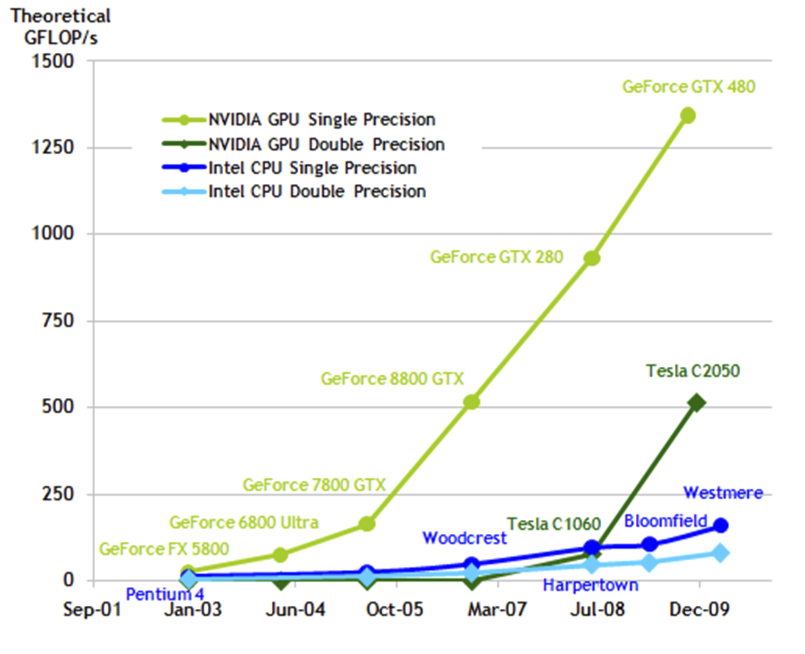
\includegraphics[width=0.7\textwidth]{images/evolucion-gpu.png}
	\caption{Comparativa de la evolución de los GFlops de las GPUs frente a las CPUs\cite{nvidia:cuda_c_programming_guide}}\label{fig:GPUvsCPU}
\end{figure}

La principal razón por la que el uso de GPU para computación se ha convertido en algo de interés es la publicación de APIs como CUDA y OpenCl que nos permiten aprovechar las capacidades de las actuales tarjetas gráficas para realizar cálculos y operaciones muy costosas en tiempo de CPU de forma más rápida. Además, permiten un alto grado de paralelismo, lo que puede resultar beneficioso para el desarrollo de ciertos tipos de programas.

En la actualidad, mientras con una CPU se podía conseguir hasta 80 millones de claves MD5 por segundo (aplicando muchas optimizaciones a nivel de lenguaje ensamblador), una GPU potente puede alcanzar hasta cerca de los 2.000 millones de resúmenes por segundo. Esto es, una GPU es hasta 250 veces más rápida que la CPU para este tipo de cálculos, propiciado, principalmente, por su mayor capacidad de paralelización.

Si consideramos el hecho de que en la actualidad casi todos los nuevos equipos que se venden en el mercado disponen de aceleradoras gráficas y que es muy fácil crear una red de ordenadores zombis se debe considerar la mejora de los mecanismos de contraseña una prioridad por parte de las organizaciones. Por este motivo es importante disponer de herramientas que permitan comprobar la fortaleza de las contraseñas y evaluar la dificultad de realizar ataques a los distintos algoritmos de resumen existentes y en experimentación.

\section{Motivación}

Como ya se ha comentado, es importante garantizar la calidad de los algoritmos que se utilizan en seguridad y las contraseñas empleadas dentro de las organizaciones. Por este motivo nace este proyecto fin de carrera que pretende ser el inicio de una herramienta versátil, sencilla y atractiva que permita ofrecer a las distintas organizaciones un mecanismo para fortalecer su seguridad. Por otra parte, el estudio del uso de tarjetas gráficas fuera del ámbito de los videojuegos y del diseño gráfico es de gran interés por la alta capacidad de cómputo que ofrecen éstas. De este modo se pretende garantizar que la amortización de los equipos informáticos es máxima ya que el aprovechamiento de los mismo será mayor. Hay que recordar que en la actualidad todos los ordenadores disponen de tarjetas gráficas con aceleración 3D y de las 3 grandes marcas del mercado (Intel, AMD y NVIDIA), dos de ellas ofrecen desde hace unos años la capacidad de ejecutar código de usuario en las mismas. En el caso de Intel, no se ofrece el uso de su GPU para cálculo, pero si permiten programar utilizando OpenCl (ver el capítulo~\ref{cap3}) para sus procesadores.

Por otra parte, la popularización de \emph{frameworks} orientados a MVC han revolucionado el mundo de la programación web. Ejemplos de ello los tenemos en Ruby on Rails, DJango o CakePHP. Lo interesante de estos \emph{frameworks} es que mejoran sustancialmente las tareas de mantenimiento de los programas web ofreciendo una serie de pautas tanto en la nomenclatura de variables y tablas de las bases de datos como en la organización que deben tener los ficheros de código fuente.

\section{Objetivos}

Para poder comprobar la fortaleza de una contraseña dada y para poder evaluar la resistencia frente a ataques de fuerza bruta de diferentes tipos de funciones resumen hace falta disponer de una herramienta adecuada. Para este fin existe una gran cantidad de herramientas, principalmente destinadas a la recuperación de contraseñas extraviadas, pero que su código es cerrado y su precio elevado. Aunque el precio puede no resultar un problema importante, consideramos que el uso de aplicaciones que no suministran su código fuente no es recomendable en el ámbito de la seguridad informática ya que es importante poder saber qué es lo que la herramienta hace y eso solo se puede determinar de forma fehaciente si ésta es de código abierto. Por otra parte, también es recomendable que la herramienta se software libre porque así, en caso de que el fabricante deje de dar soporte a la misma, tendríamos permiso para poder realizar modificaciones eliminando de este modo la dependencia con el vendedor.

El presente proyecto final de carrera nace con el objetivo de aprovechar las nuevas arquitecturas gráficas en el entorno de la evaluación de seguridad informática, especialmente en el ámbito de las funciones resumen. Igualmente se ha pretendido utilizar un modelo distribuido para mejorar la escalabilidad del sistema y así disponer de una herramienta potente que pueda ser ampliada según la necesidad del momento.

En concreto, los objetivos que se pretenden alcanzar con la realización de este proyecto son:

\begin{description}

	\item[Estudio de las distintas técnicas de evaluación de contraseñas.] Para poder garantizar la calidad de cualquier solución planteada para la evaluación de contraseñas es necesario disponer de una base suficiente sobre el tema. De este modo será más sencillo determinar si el trabajo realizado es correcto o no.
	
	\item[Aprendizaje de programación con GPU.] Esto permitirá hacer uso de un elemento de gran potencia que se encuentra hoy día en todos los ordenadores comercializados. Además, las GPU ofrecen unas características ideales para la ejecución de una gran cantidad de tareas en paralelo lo que las hace muy atractivas para realizar tareas que de otro modo podrían tardar muchísimo.
	
	\item[Utilizar nuevas técnicas de distribución de tareas.] A lo largo de la carrera se ha tratado en muchas ocasiones los sistemas distribuidos y cómo estos distribuyen su carga de trabajo entre una red de ordenadores. En este punto se pretende experimentar con algunas técnicas no tratadas o con mecanismos diferentes a los vistos.
	
	\item[Aplicar técnicas de usabilidad.] Un apartado importante de toda aplicación es la facilidad con la que esta se maneje y el grado de satisfacción del usuario de la misma. Por este motivo es importante dedicar un esfuerzo en el diseño de la interfaz y así mejorar la experiencia del usuario.
	
	\item[Ofrecer una buen grado de escalabilidad.] Gracias a esto se pretende conseguir que el sistema desarrollado puede crecer con el tiempo de forma sencilla introduciendo nuevos ordenadores. De este modo se reducirían los costes al no tener que comprar grandes sistemas exclusivamente para este propósito.
	
	\item[Garantizar que la herramienta desarrollada sea mantenible.] Para ello es necesario hacer un buen uso de los comentarios y se debe garantizar que estén bien documentados los aspectos más importantes de diseño de la herramienta. De este modo se conseguirá que en un futuro cualquier persona puede realizar modificaciones sobre la misma en caso de fallos.
	
	\item[Implementar un sistema de extensiones.] Con esto se pretende que la herramienta pueda ver ampliada su funcionalidad sin necesidad de que deba ser compilada nuevamente. Para ser más exactos, lo que se pretende es que durante el inicio de la ejecución de la herramienta esta busque en el sistema extensiones que le añadan funcionalidades.
	
	\item[Crear un mecanismo sencillo de administración.] De este modo se pretende mejorar el tiempo requerido para la realización de las tareas relacionadas con la aplicación.
	
	\item[Desarrollo de una interfaz web.] En la actualidad casi todos los equipos informáticos se encuentran conectados, sino a Internet, sí a una red de ordenadores. Por norma general los cortafuegos empresariales filtran el tráfico que circula por la red, pero permiten el uso de Web lo que convierte a la Web casi en el medio exclusivo para usarlo como protocolo para la administración remota.
	
	\item[Uso de los \emph{frameworks} MVC.] Con esto se pretende garantizar la mantenibilidad de la solución web anteriormente comentada. Además, el uso de \emph{frameworks} ya existentes facilitan el mantenimiento de la aplicación ya que solo habrá que dedicar esfuerzo al desarrollo de la herramienta y en caso de mejoras en el \emph{framework} éstas se pueden ver inmediatamente reflejadas en la aplicación sin apenas tener que realizar cambios (en muchos casos no es necesario realizar cambio alguno).
\end{description}

\section{Estructura del documento}

Para facilitar la búsqueda a través del este documento, se provee de la siguiente guía de la organización interna del mismo. Éste se divide en los siguiente capítulos:

\begin{description}
	\item[Funciones resumen:] introducción a las funciones resumen y a los tipos de ataques que existen sobre ellas. Es importante comprender qué son para entender mejor cuales son los objetivos del proyecto.
	
	\item[Desarrollo con tarjetas gráficas:] se introduce la historia del desarrollo con tarjetas gráficas y a cómo se programa utilizando CUDA, el API de NVIDIA. Con esto se pretende ofrecer una visión global sobre el uso de tarjetas gráficas y el porqué de su uso.
	
	\item[Mejora de una aplicación distribuida:] se muestra un estudio sobre una aplicación ya existente y los cambios que se le han realizado y las motivaciones para ello.
	
	\item[Resultados:] se enumeran las pruebas y los resultados obtenidos por las mismas.
	
	\item[Conclusiones:] conclusiones obtenidas de la realización del proyecto en las que se intenta valorar el grado de consecución del mismo.
	
	\item[Trabajos futuros:] descripción de posibles trabajos futuros que sería interesante realizar a partir del trabajo realizado en este proyecto final de carrera.
\end{description}
	\chapter{Funciones resumen}\label{cap2}

Los sistemas destinados a ocultar o proteger información llevan usándose desde tiempos de la antigua Roma \cite{Luciano87cryptology:from} e incluso antes. Paralelamente se ha tratado siempre de crear las técnicas necesarias para poder acceder a dicha información sin ser el destinatario legítimo de la misma. Esto ha creado la necesidad de mejorar constantemente los mecanismos de cifrado para evitar que la información protegida no pueda ser utilizada salvo por aquellos a la que está destinada.

En la actualidad hay una gran cantidad de sistemas para la protección de información y se utilizarán unos u otros dependiendo de lo que se pretenda hacer. Concretamente existen 3 grandes grupos de mecanismos de seguridad:
\begin{itemize}
	\item Sistemas de cifrado de clave simétrica, que son aquellos que utilizan una clave para cifrar la información y esta clave debe ser conocida por todos aquellos que quieran tener acceso a información.
	\item Sistemas de cifrado de clave asimétrica, que utiliza dos juegos de claves, una pública y conocida por todo el mundo y otra privada que solo su propietario posee.
	\item Sistemas de un solo sentido o funciones resúmenes (también conocidas como funciones \emph{hash}).
\end{itemize}

Las funciones resumen, que son las que nos interesan para el presento proyecto fin de carrera, son aquellas que cumplen las siguientes características:

\begin{itemize}
	\item Son fáciles de calcular en un sentido, pero es muy complicado hallar su inversa y
	\item Que dada una entrada de longitud arbitraria siempre producirán una salida de longitud fija.
\end{itemize}

Este tipo de funciones son ampliamente utilizadas en el mundo de la seguridad como sistema para el almacenamiento de contraseñas de usuario, la generación de claves de sesión o la firma digital de documentos (por poner algunos ejemplos). Al ser ampliamente utilizadas es importante disponer de mecanismos para comprobar la fortaleza del mecanismo de funcionamiento como la fortaleza de la clave elegida.

A causa de su gran uso es necesario disponer de sistemas que comprueben la fortaleza de las contraseñas elegidas por los usuarios o de las claves de sesión que pueda generar un sistema de seguridad. El primer caso es importante para garantizar la seguridad de las organizaciones, impidiendo que los usuarios elijan contraseñas que puedan ser adivinadas o quebrantadas por posibles atacantes dando acceso a la información privada de ésta con los consiguientes problemas por posibles copias y/o borrados de información. El segundo caso es importante para garantizar que los sistemas seguros sean capaces de generar claves suficientemente robustas para impedir ataques externos.

\section{Comprobación de funciones resumen y contraseñas}\label{sec:comprobacion_resumen}

Existen dos formas básicas para comprobar la fortaleza de los mecanismos de seguridad. El primero es buscar debilidades en la propia función resumen que se va a utilizar. El segundo mecanismo es comprobar la calidad de la clave utilizada. Para este último caso lo más sencillo es utilizar un de mecanismo de fuerza bruta. Éste tipo de comprobación consisten en probar todas las combinaciones posibles entradas para generar resúmenes y éstos se cotejan con un resumen conocido previamente.

El mayor problema de los sistemas de fuerza bruta es el tiempo que tardan en ofrecer algún resultado. Esto se debe a la gran cantidad de comprobaciones que deben realizar. Por este motivo es importante poder predecir el tiempo que dedicarán previamente para comprobar si vale o no la pena intentar realizar una comprobación de éste tipo.

Para poder calcular el tiempo que se necesitará para poder poder hacer una comprobación de fuerza bruta empezaremos por el caso genera. En éste, el tiempo máximo (el que recorre todas la combinaciones posibles) es de:

$$ T_{max}=t\sum^n_{i=m}k^i $$
 
Donde $m$ es la longitud mínima de la entrada, $n$ es la longitud máxima y $k$ es el número de símbolos posibles del alfabeto a utilizar. Finalmente $t$ representa el tiempo de cómputo de la función resumen.

Utilizando este sistema como referencia de peor caso es fácil medir las mejoras aportadas por otros algoritmos. De este modo, y tomando como referencia el trabajo realizado en este proyecto final de carrera, el simple uso de la paralelización utilizando un sistema de $C$ procesadores homogéneos nos proporciona unos tiempos de:

$$ T_{max}=t\sum^n_{i=m}\frac{k^i}{C} $$

En la actualidad, gracias a los avances en las comunicaciones y a los distintos procesadores es normal disponer de sistemas distribuidos heterogéneos. Éstos pueden contar con unas cuantas máquinas o cientos de miles. Para este tipo de casos es necesario disponer de una función general que tenga en cuenta la velocidad de cálculo en cada tipo de procesador en que vaya a ejecutarse la función resumen. Si disponemos de $p$ tipos de procesadores distintos y $C_j$ procesadores para cada tipo que tardan $t_j$ segundos en computar la función resumen ($1 \leq j \leq p$):

$$ T_{max}=\frac{\sum^n_{i=m}k^i}{\sum^p_{j=1}\frac{C_j}{t_j}}$$
 
Con esta información  se puede calcular cuál debe ser el tamaño del sistema a utilizar para poder comprobar la fortaleza de una contraseña en un tiempo determinado.

Por ejemplo, si dispusiéramos de un sistema con las siguientes características:

\begin{itemize}
	\item 4 microprocesadores capaces de hacer 25 millones de resúmenes por segundo cada uno.
	
	\item 4 tarjetas gráficas capaces de hacer 1.250 millones de resúmenes por segundo cada una.
\end{itemize}

Tardaríamos unas 9,5 horas en encontrar una contraseña de entre 6 y 8 caracteres utilizando solo letras minúsculas y números. Es importante tener en cuenta que al buscar una contraseña se puede acotar mucho el conjunto de símbolos de entreda y las longitudes de las claves. Esto reduce enormemente los tiempos de búsqueda.
%Por otra parte sabemos que la longitud de las contraseñas está entre 6 y 8 caracteres de longitud y que el usuario solo utiliza letras minúsculas y números.
%2 tipos de procesadores diferentes para calcular una función resumen y que el primer procesador puede hacer una media de 25 millones de resúmenes por segundo y el segundo procesador puede hacer 1250 millones de resúmenes por segundo (éste caso se aproxima al uso de CPU+GPU). De cada procesador se dispone de 4 unidades. Además, nuestra clave está entre 6 y 8 caracteres de longitud y solo vamos a considerar letras minúsculas y números lo que supone 36 símbolos de entrada. Esto supone que el tiempo máximo que tardará el sistema en comprobar todas las combinaciones en las condiciones expuestas es de casi 9,5 horas.

Es fácil comprobar que utilizando sistemas de fuerza bruta para comprobar resúmenes se resuelve de forma lineal con respecto al número de procesadores.

A parte de los sistemas de fuerza bruta, existen muchas técnicas que han surgido a partir de la investigación de los distintos tipos de sistemas de resumen. Estos nuevos sistemas proceden de debilidades de los propios algoritmos y deben ser tenidos en cuenta a la hora de evaluar la fortaleza de las funciones resumen.

Aunque no es propósito del presente proyecto de fin de carrera implementar todos los sistemas de comprobación conocidos sí es importante tenerlos en cuenta para poder hacer comparaciones y valoraciones con respecto a las soluciones implementadas.

\subsection{Ataque de cumpleaños}

Este ataque a los sistemas de resúmenes consiste en que dado un mensaje $M$ cualquiera y una función resumen $H$, que genera resúmenes de longitud $L$ bits, se puede hallar un mensaje $M’$ probando combinaciones aleatorias en aproximadamente $1.2\sqrt{2^L}$ intentos \cite{website:wastahf} \cite{Oorschot:1994:PCS:191177.191231}(en caso de que la función resumen sea uniformemente distribuida).

El principio en el que se base este ataque se encuentra en un problema de teoría de la probabilidad conocido como problema del cumpleaños o paradoja del cumpleaños. Esta dice que un grupo de personas debe tener 23 individuos para que haya un 50\% de probabilidad de que dos cumplan hayan nacido el mismo día (figura \ref{fig:Birthday}).

El funcionamiento general es el siguiente:

$$
P(i, n) = \left\{
	\begin{array}{l l}
		1                        & \mbox{si $i = 1$}\\
		P(i-1, n)\frac{n-i+1}{n} & \mbox{si $i > 1$}
	\end{array} \right.
$$

Donde $P(i, n)$ es la probabilidad de que para una población final de $n$ elementos (365 en el caso de los cumpleaños) y disponiendo de $i$ elementos seleccionados aleatoriamente dos individuos no coincidan. Por ejemplo, si tomamos tres individuos aleatoriamente el primero de ellos habrá nacido un día cualquiera del año (la probabilidad de que dos individuos no cumplan años el mismo día es del 100\% ó $365/365$), el segundo habrá nacido uno de los restantes días ($364/365$) y el tercero igual ($353/365$). La probabilidad total será el producto de las probabilidades; en este caso concreto es de $0.9945$.

Este mismo principio es aplicable a las funciones resumen \cite{Bellare04hashfunction}, ya que se puede considerar que en lugar de días del año tenemos resúmenes (todas las posibles combinaciones de éstos) y en lugar de personas tenemos textos o mensajes a ser cifrados.

En el caso de las funciones resumen hay que tener en cuenta la distribución que hacen éstas de los datos de entrada ya que las funciones no uniformes serán en las que es más sencillo encontrar colisiones (se puede centrar la búsqueda en los cúmulos). Esto supone que en lugar de tener probar combinaciones aleatorias diferentes podríamos reducir el número intentos.
 
\begin{figure}
	\centering
	\includegraphics[width=0.7\textwidth]{images/happybirthday.pdf}
	\caption{Probabilidad de encontrar dos personas nacidas el mismo día con respecto al tamaño del grupo}\label{fig:Birthday}
\end{figure}

Estas características del sistema del cumpleaños lo convierten en un sistema ideal para sustituir a los mecanismos de fuerza bruta convencionales, pero hay que tener en cuenta que se debe considerar el tiempo de crear los mensajes a probar (dependiendo de su longitud podría hacer al sistema igual de rápido que uno de fuerza bruta) y el tamaño de la muestra; el principal problema del ataque de cumpleaños es que debe trabajar sobre todas las posibles combinaciones existentes lo que puede suponer un problema en casos en los que sepamos que hay una gran cantidad de restricciones. Por ejemplo, en el caso expuesto al inicio de la sección en el que se tardaba 9,5 horas en completar la búsqueda se tardaría cerca de 8.217,73 años utilizando este mecanismo. Esto significa que hay que estudiar el problema para poder descubrir las debilidades locales (en el caso de las contraseñas puede ser la longitud, el conjunto de caracteres posibles, etc.).

\subsection{Tablas arcoíris}

Las tablas arcoíris son una técnica por la que se toma un conjunto de entradas y sobre cada una de éstas se realizan un proceso iterativo de resúmenes que van tomando el último resumen realizado para hacer uno nuevo hasta obtener un elemento que consideraremos terminal. Se puede considerar este proceso como una tabla en el que la primera columna son las distintas entradas que se han elegido y cada columna $C_j$, para $j>1$, representa el resumen de la columna anterior ($C_j = H(C_{j-1})$, ver cuadro \ref{tab:arcoiris}). La tabla arcoíris consiste en tomar la primera y última columnas.

\begin{table}
	\centering
	\begin{tabular}{ccccc}
		$M$   & $H(M)$ & $H(M')$ & $H(M'')$ & $H(M''')$\\
		\hline
		$m_1$ & $m'_1$ & $m''_1$ & $m'''_1$ & $m_{1,terminal}$\\
		\hline
		$m_2$ & $m'_2$ & $m''_2$ & $m'''_2$ & $m_{2,terminal}$\\
		\hline
		$m_3$ & $m'_3$ & $m''_3$ & $m'''_3$ & $m_{3,terminal}$\\
		\hline
		$m_4$ & $m'_4$ & $m''_4$ & $m'''_4$ & $m_{4,terminal}$\\
		\hline
	\end{tabular}
	\caption{Ejemplo de tabla arcoíris}\label{tab:arcoiris}
\end{table}

Una vez que se dispone de la tabla arcoíris se pueden empezar a probar claves por fuerza bruta y si en algún momento alguna coincide con algún elemento final de la tabla arcoíris simplemente tenemos que buscar los resúmenes empezando en el que genero dicho elemento terminal (el mensaje inicial).

El principal problema de éste sistema es determinar el tamaño de la tabla a utilizar y el tiempo que se necesita para crearla. En general este mecanismo solo se utiliza para casos muy concretos de funciones resumen débiles.

\subsection{Caminos diferenciales para SHA-1}\label{sub:sha1}

La técnica de los caminos diferenciales consiste en realizar una estudio sobre los cambios en los bits de las variables utilizadas en una función resumen. El objetivo es detectar estadísticamente los puntos en los que se producen alternancia de bits o en los que éstos no cambian para realizar una aproximación estadística a posibles colisiones.

En \cite{citeulike:7684257} se puede encontrar un estudio que a partir del uso de aproximaciones no lineales es capaz de encontrar una colisión en SHA-1 en $2^{52}$ intentos. Para ello toma el resumen para el que deseamos hayar un mensaje que lo genere y trata de determinar los mensajes que pudieron haberlo generado deshaciendo el algoritmo tomando los datos de los posibles cambios obtenidos en el estudio anteriormente comentado.

Como sucedía con el ataque del cumpleaños, esta técnica es interesante siempre y cuando el conjunto de caracteres de entrada sea completo ya que en el caso de de contraseñas, donde se utiliza un juego de caracteres muy limitado, una técnica de fuerza bruta puede resultar más eficiente.



	\chapter{Desarrollo con tarjetas gráficas}\label{cap3}

\section{Breve historia de la computación con GPUs}

Desde hace bastante tiempo se lleva usando las capacidades de las tarjetas gráficas para realizar computación. Concretamente se han utilizado para la realización de efectos sobre texturas y polígonos con la tecnología denominada \emph{shaders}. Estos \emph{shaders} son pequeños programas que transforman la forma de verse los puntos o como se transforman los polígonos y que se han estado ejecutando en las GPUs para mejorar su rendimiento.

A partir de esta tecnología y tras numerosas especulaciones sobre las capacidades de las tarjetas gráficas para realizar cálculos más genéricos, las compañías empezaron a abrir sus sistemas para permitir cargar códigos orientados a cualquier tipo de cálculo matemático.

Los primeros productoos con este tipo de tecnología provinieron de BionicFX y fueron presentados a principios de 2005 \cite{website:extremetech_gpu_audio}. En este caso se hacía uso de gráficas con GPU NVIDIA para procesador de audio. Para ello transformaba el sonido en datos gráficos y luego éstos se procesaban con los medios matemáticos de que disponía la GPU.

Más tarde, en el año 2006, la compañía AMD anuncia la comercialización de AMD Stream Processor~\cite{website:amd_press_stream}, el primer sistema de cálculo basado en tarjetas gráficas. De este modo se empezó a comercializar el primer sistema que realmente permitía cargar código de usuario en la tarjeta para realizar cálculos que no estuviesen directamente relacionados con generación de imagen en 3D.

La compañía NVIDIA publica el 15 de febrero de 2007 la bibliotecas CUDA~\cite{website:nvidia_press_cuda} que permite usar sus tarjetas gráficas para cálculo y, además, comercializa la arquitectura Tesla que, como en el caso de ATI, es un sistema específico de cálculo basado en tarjetas gráficas.

En base a esta popularización del cómputo con tarjetas gráficas y por  su utilizad gran utilidad para todo tipo de procesos (especialmente aquellos destinados a multimedia e investigación), Apple publica un borrador de OpenCl (Open Computing Language) y posteriormente éste es pasado a control de Khronos Group~\cite{website:khronos_press_opencl}. OpenCl es  el primer estándar creado específicamente para cómputo distribuido, orientado principalmente a GPUs, y que ofrece una interfaz común para todo tipo de tarjetas gráficas y otros sistemas de cálculo (como procesadores multinúcleo, FPGAs, procesadores CELL, etc.). Esta tecnología solo se incluye de serie en el sistema operativo Apple Mac OS X 10.6, pero fabricantes como ATI y NVIDIA proveen de controladores para otras plataformas.

El mecanismo más eficiente para aprovechar las capacidades de una tarjeta gráfica es utilizar la API del fabricante ya que éste está optimizado para aprovechar mejor la arquitectura. Esto supone que en casos en los que la eficiencia es algo absolutamente crítico sea mejor opción frente al uso de la biblioteca OpenCl.

Estos sistemas están teniendo mucha relevancia debido a su alto rendimiento, especialmente en aplicaciones científicas. Además, se han realizado avances en el desarrollo de aplicaciones específicas de ruptura de contraseñas.

En la actualidad la computación con tarjetas gráficas está empezando a utilizarse en todo tipo de cálculos, tanto para investigaciones científicas  como para herramientas de usuario como descompresores de vídeo y audio, filtros gráficos en herramientas de diseño o videojuegos. Todo esto gracias a las grandes capacidades de paralelización de cálculos de las GPUs como a la faciliad de realizar cálculos vectoriales de forma sencilla. Esto significa que es una tecnología apoyada por la industria y que se va a disponer de soporte y documentación para realizar desarrollos con la misma.

Se puede comprobar, además, como en el año 2008 empezaron a surgir los primeros sistemas orientados a la seguridad informática que se apoyaban en el uso de tarjetas gráficas para realizar dicha función. Un ejemplo de esto lo tenemos en la herramienta de Elcomsoft publicada en octubre de 2008~\cite{website:elcomsoft_press} que hace uso de tarjetas gráficas para recuperar contraseñas.

\section{Introducción a CUDA}

Para desarrollar este proyecto se ha hecho uso de la tecnología CUDA de NVIDIA por varios motivos:
\begin{itemize}
	\item Las tarjetas gráficas NVIDIA están muy distribuidas y vienes de serie en la mayor parte de equipos informáticos de gama media/alta.
	\item El uso de un API específico ayuda a aprovechar mejor las características de la arquitectura frente a un API más general como pueda ser OpenCl.
	\item En el momento de realizar este proyecto se dispone de un sistema NVIDIA Tesla, por lo que CUDA se convierte en la solución ideal.
\end{itemize}

A la hora de desarrollar en una nueva arquitectura es importante conocer las características de la misma. Estas características pueden ir desde cómo se gestiona la memoria, qué instrucciones posee, etc.

\subsection{Arquitectura}

Las tarjetas gráficas NVIDA disponen de una gran cantidad de unidades aritmetico-lógicas (figura~\ref{fig:cudaorggpu}) para poder realizar una mayor cantidad de cálculos por ciclo de reloj~\cite{nvidia:cuda_c_programming_guide}. Gracias a esto las tareas que hacen usos de cálculos intensivos pueden verse muy beneficiadas. Por otra parte, las GPU disponen también de un gran número de unidades de control lo que permite disponer de una gran número de tareas en paralelo. La combinación de las dos características anteriores es lo que dota a las tarjetas gráficas de una gran capacidad para ejecutar algoritmos en paralelo.

\begin{figure}
	\centering
	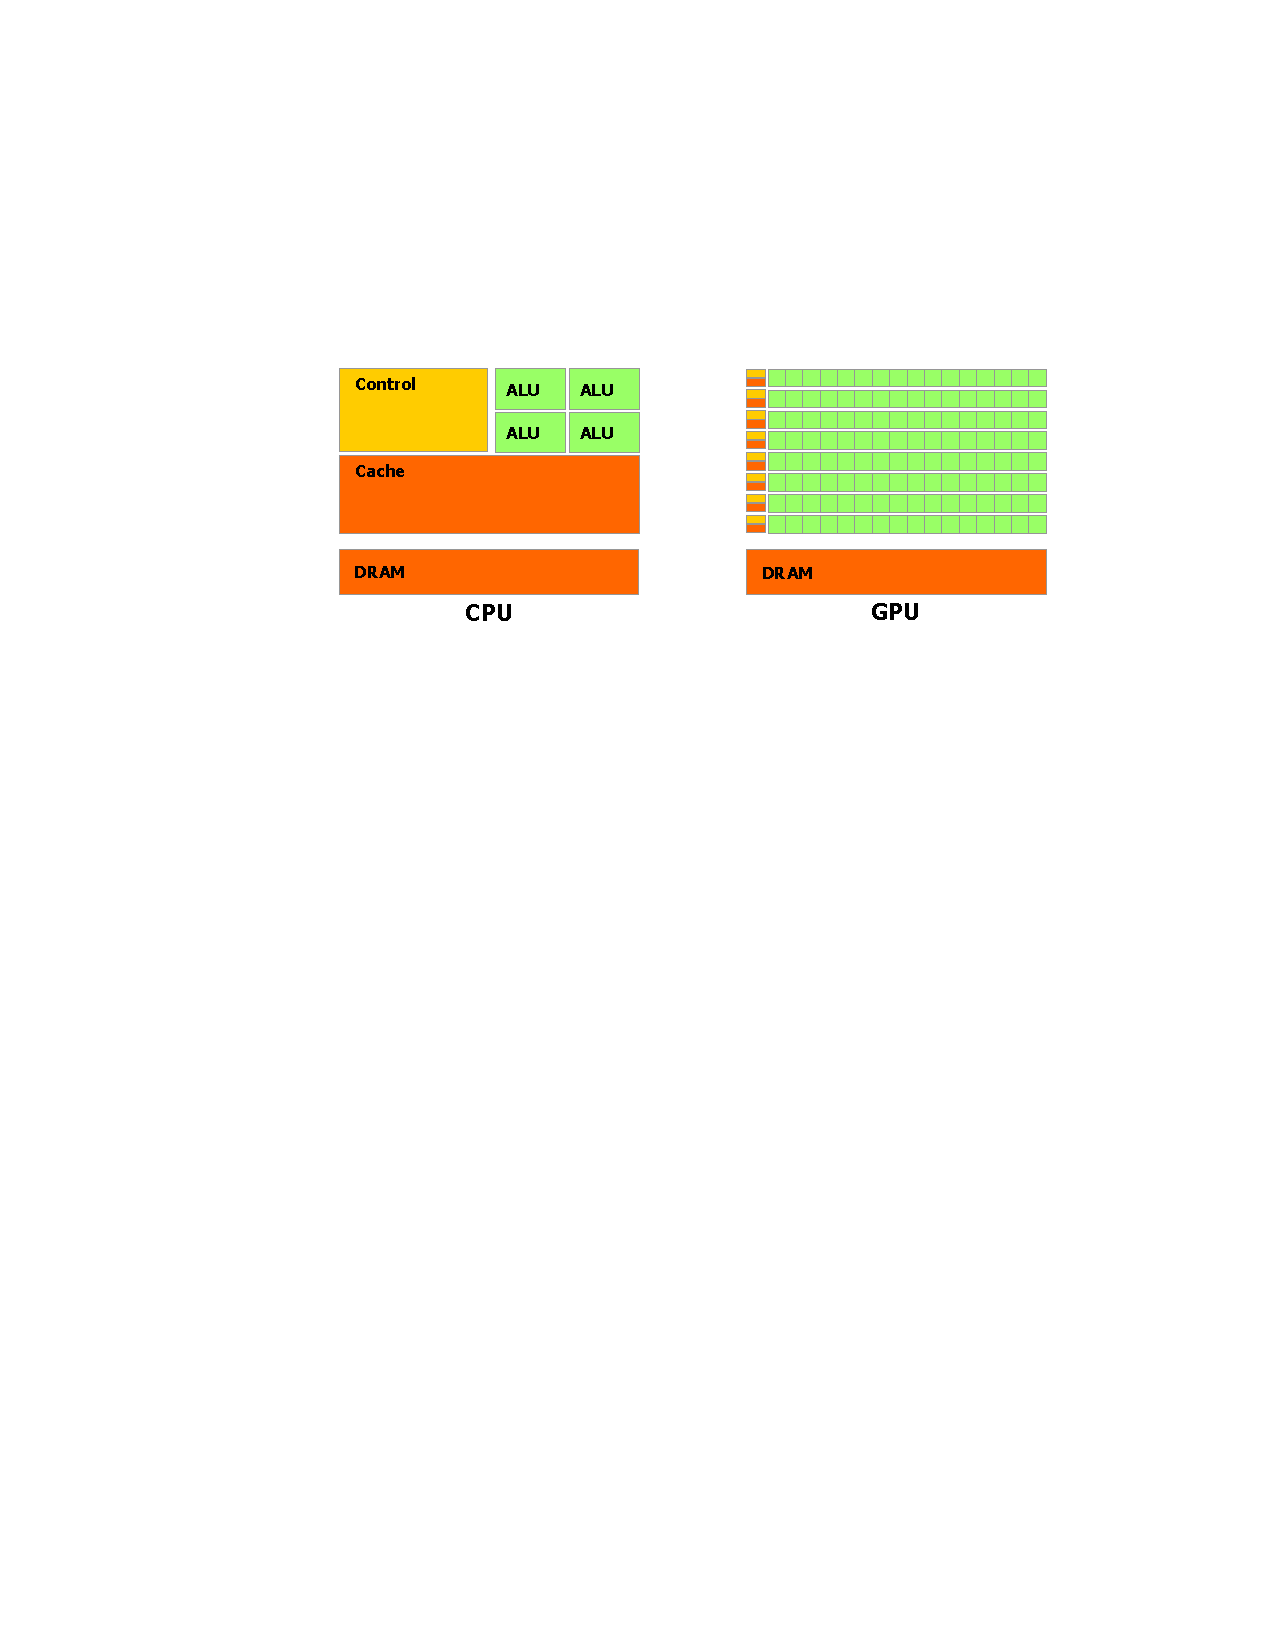
\includegraphics[width=1\textwidth]{images/cpuvsgpu.pdf}
	\caption{Comparativa de organización de CPU y GPU \cite{nvidia:cuda_c_programming_guide}}\label{fig:cudaorggpu}
\end{figure}

Además de como está organizada la GPU, es importante tener en cuenta como se organiza la memoria (figura~\ref{fig:memcuda}) ya que el buen uso de ésta influirá de forma muy significativa en el rendimiento de los programas. Esta arquitectura es la misma que la de las tarjetas gráficas y se puede representar como una pirámide de tiempos dependiendo del tipo de memoria a la que se vaya a acceder.

La memoria de sistema es la que se encuentra en el equipo sin contar la que aporta la tarjeta gráfica. Los programas de ordenador puede hacer uso de ésta de forma sencilla, pero los programas que se ejecutan dentro de la GPU no puede acceder a ella. Tanto la memoria global como la memoria de textura se encuentran en la tarjeta gráfica y servirán de almacen de los datos que requieran los programas que se hallen en ésta. La principal diferencia entre ambas reside en el modo a través del cual se accede a ellas. La memoria global funciona igual que la memoria de sistema para un programa normal (a partir de un puntero se accede a la misma), mientras que la memoria de textura se accede haciendo uso de un sistema especial que añade funcionalidades como interpolado. La ventaja de la memoria de textura es que dispone de un acceso más rápido (se debe a que es guardada en caché) lo que la convierte en muy una opción muy atractiva para cierto tipo de cálculos.

Por último, los registros de la GPU dispone de un acceso muy rápido por lo que es recomendable hacer uso de los mismos siempre que sea posible.

\begin{figure}
	\centering
	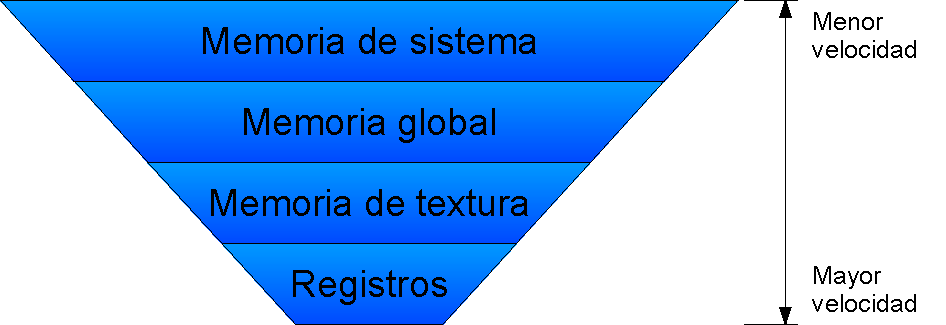
\includegraphics[width=0.7\textwidth]{images/MemoriaCuda.pdf}
	\caption{Jerarquía de memoria en CUDA}\label{fig:memcuda}
\end{figure}

La optimización del uso de la memoria es fundamenta para mejorar el rendimiento de las aplicaciones CUDA ya que si se trabaja con una cantidad muy grande de datos se puede perder una parte importante de tiempo realizando copias de memoria. Por este motivo hay que realizar un buen estudio sobre el uso que se va a realizar de la memoria.

\subsection{Modo de desarrollo}

Para programar para CUDA es muy importante tener en cuenta cómo se organiza la ejecución del código ya que influirá en la forma en la que habrá que diseñar nuestros algoritmos. De éste modo, los códigos que se ejecutan en la tarjeta gráfica se organizarán del siguiente modo:

\begin{description}
	\item[\emph{threads}] que son tareas que se ejecutan en paralelo y que comparte código. Los \emph{threads} se organizan de forma tridimensional de tal modo que podría haber momento en los que un \emph{thread} estuviese encima, debajo o al lado de otro.
	\item[\emph{blocks}] que son grupos de \emph{threads} y al igual que éstos también se se organizan de forma tridimensional. Todos los \emph{threads} contenidos en un \emph{block} se ejecutarán al mismo tiempo, de modo que si la GPU no tiene capacidad para el total de \emph{threads} solicitados por \emph{block} devolverá un error.
	\item[\emph{grid}] que es un conjunto de \emph{blocks}. Los \emph{grids} se organizad en planos, esto es, solo dispone de 2 dimensiones.
\end{description}

En la figura~\ref{fig:cudaorg} puede verse de forma más clara la organización de los \emph{threads}. Es importante tener en cuenta que, como se ha dicho, todos los \emph{threads} de un \emph{block} se ejecutan a la vez, pero los \emph{blocks} no tienen porque hacerlo. Este detalle es importante a la hora de ajustar el acceso a la memoria ya que cuando un \emph{thread} accede a ésta podrá verse optimizado si lo hace de forma ordenada con el resto de \emph{threads} del \emph{block}.

\begin{figure}
	\centering
	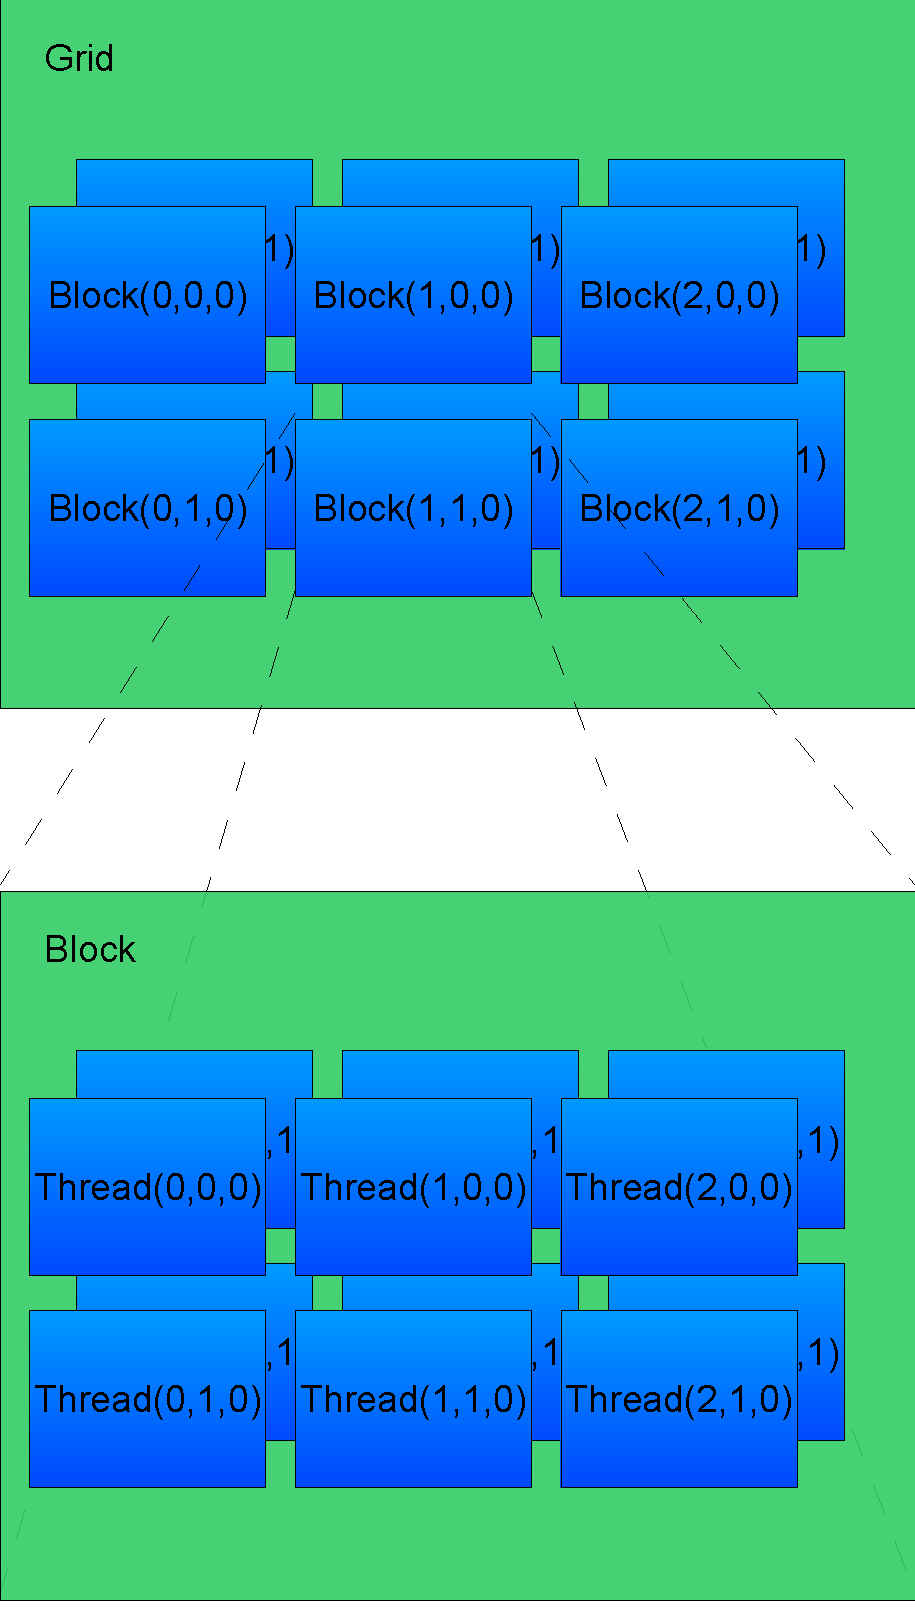
\includegraphics[width=0.7\textwidth]{images/cuda_org.pdf}
	\caption{Organización de procesos en ejecución en CUDA}\label{fig:cudaorg}
\end{figure}

Otro aspecto muy importante a tener en cuenta es la organización del acceso a memoria. Como ya se vio en el apartado anterior, ésta está organizada de forma jerárquica según la velocidad de acceso. Además, también es importante tener en cuenta como los \emph{threads} acceden a la memoria ya que si lo hacen de manera organizada se puede conseguir incrementos de rendimiento. Esta último se debe a que, si por ejemplo todos los \emph{threads} acceden a posiciones contiguas de memoria (el primer \emph{thread} lee el primer elemento de la memoria, el segundo \emph{thread} lee el segundo elemento, etc.) se consigue que todas las lecturas de todos los \emph{threads} se realicen en paralelo. Por el contrario, si las lecturas se hacen de forma desordenada éstas se realizarán de forma secuencia, malgastando de este modo un tiempo precioso.
 
Como la memoria del sistema es inaccesible para los \emph{threads} es importante tener en cuenta que solo se podrá utilizar la memoria de la tarjeta gráfica. Esto supone que antes de realizar operaciones sobre memoria en CUDA hay que reservar la memoria a utilizar e inicializarla desde el programa principal que se encuentra en la CPU. Esta inicialización suele realizarse en tres tiempos:

\begin{enumerate}
	\item En un primer momento se preparan los datos que se pasarán a la GPU.

	\item Seguidamente se reserva la memoria en la tarjeta gráfica

	\item Por último se copian los datos a la tarjeta gráfica para poder ser usados desde la parte que será ejecutada en la GPU.
\end{enumerate} 

Por otra parte hay que tener en cuenta que una vez se disponen de los datos sobre la memoria de la tarjeta gráfica es importante estudiar si conviene utilizarlos desde dicho punto o si es preferible realizar una copia a registros de procesador que serán mucho más rápidos. La tarjeta gráfica provee de una gran cantidad de registros (hasta 16.384 en el caso de las NVIDIA Tesla) para poder acelerar los cálculos por lo que hay que se deberá hacer uso de los mismos en la medida de lo posible. De este modo, si la cantidad de operaciones a realizar va a ser muy elevada, compensa el tiempo que se dedicará a copiar los datos desde la memoria de la tarjeta gráfica a los registros.

Por norma general, todo código que vaya a ser alojado en una GPU se seguirá un patrón de ejecución como el descrito a continuación (figura~\ref{fig:procejecuda}):

\begin{itemize}
	\item Se copian los parámetros que se hallen en memoria global a registros, siempre que sea posible, para acceder a los mismos desde ahí. Esto es especialmente importante si el número de accesos va a ser elevado ya que de otra forma se estaría desperdiciando una gran cantidad de tiempo en realizar accesos a memoria.
	\item Una vez que ya se tiene la memoria iniciada se procede a realizar los cálculos oportunos.
	\item Finalmente se preparan los resultados para ser volcados a la memoria global de la tarjeta gráfica y que de este modo puedan ser leídos por la aplicación.
\end{itemize}

\begin{figure}
	\centering
	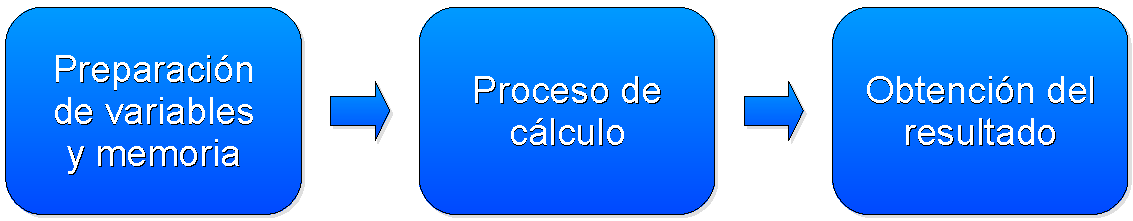
\includegraphics[width=0.7\textwidth]{images/proc_ejec1.pdf}
	\caption{Proceso de ejecución de un algoritmo en CUDA}\label{fig:procejecuda}
\end{figure}

El \emph{kit} de desarrollo de CUDA ofrece dos formas diferentes de realizar desarrollar aplicaciones. En la primera forma, la más sencilla, CUDA se encarga de realizar las llamadas al código que se alojará en la GPU de forma transparente de tal forma que no tendremos que preocuparnos de configurar muchos de los parámetros de los que dispone el sistema. Este mecanismo es muy útil y permite un desarrollo rápido de funciones. Por otra parte estaría el sistema completo con el que debe utilizarse la API de bajo nivel de CUDA y que permite un nivel más alto de granularidad. Con este sistema nosotros deberemos de realizar a mano la carga del código en la GPU, seleccionar la GPU de todas las posibles, etc.

Con independencia del mecanismo elegido para utilizar CUDA hay algunas tareas que se deben realizar siempre de forma manual. La más importante es la administración de la memoria; cuando se va a enviar datos a la tarjeta gráfica antes de nada hay que reservar la memoria y luego se debe hacer una copia de los datos desde la memoria de sistema a la memoria que se acaba de reservar. Cuando esta área de memoria ya no se necesite se deberá liberar.

El proceso de copiar memoria desde la RAM a la tarjeta gráfica es bastante rápido gracias a los nuevos buses de comunicaciones PCI Express que está especialmente diseñados para estas labores, pero esto no evita el hecho de que si la cantidad de datos a copiar es muy grande el tiempo desperdiciado entre llamadas puede ser muy grande. Esto se hace realmente patente cuando el proceso a ejecutar es muy rápido donde se puede perder mucho tiempo realizando copias de memoria.

Por el motivo anterior CUDA provee de técnicas más avanzadas optimizar el uso de la arquitectura y mejorar la concurrencia para evitar tiempos muertos (figura~\ref{fig:cudaejecavanzada}). Éstas consisten en el uso de \emph{streams}, por un lado, y, si es posible, la reutilización de resultados previos. Los \emph{streams} son un mecanismo de comunicación con la tarjeta gráfica que permite tener varios canales de comunicaciones asociados con una llamada a función. Cuando se utiliza \emph{streams} se puede disponer de dos canales, mientras se está ejecutando una función por el primer canal ya se puede utilizar el segundo canal para cargar los datos de la siguiente ejecución. Esto permite optimizar el uso de los tiempo muerto de la CPU y se ahorra la esperar de la carga desde memoria de sistema a la memoria de la tarjeta gráfica.

\begin{figure}
	\centering
	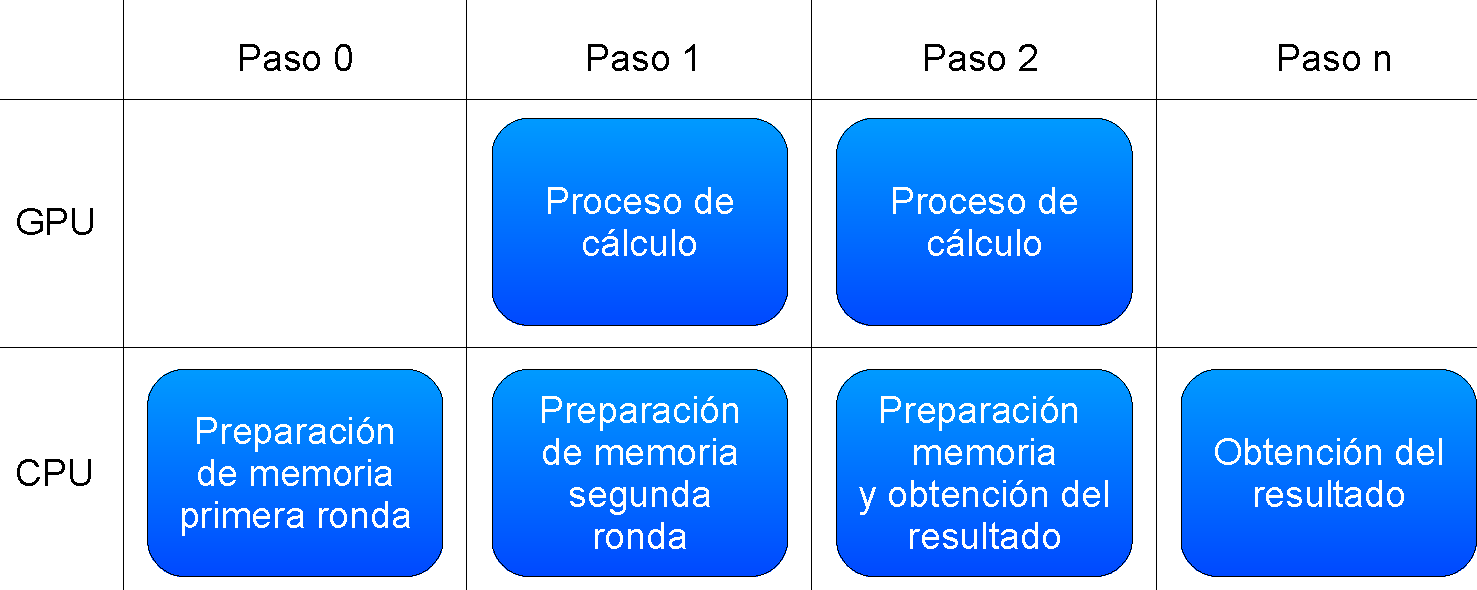
\includegraphics[width=1\textwidth]{images/ejec_gpu_complex.pdf}
	\caption{Ejecución en GPU optimizando usando streams}\label{fig:cudaejecavanzada}
\end{figure}

La reutilización de los valores previos es muy útil cuando se utilizan funcione de la forma $f(x) = af(x-1)+b$ ya que evita tener que realizar un exceso de copias de memoria. Si ya disponemos del resultado de la próxima ejecución en memoria simplemente lo dejamos ahí y lo utilizamos en lugar de copiarlo a memoria de sistema para después cargarlo a la memoria de la tarjeta gráfica.



	\chapter{Mejora de la aplicación}\label{cap4}

Para la realización de este proyecto fin de carrera se decidió buscar herramientas que hicieran uso de tarjetas gráficas para comprobar contraseñas. Tras una búsqueda exhaustiva se determina que la aplicación \emph{Distributed Hash Cracker} era la más completa y, lo más importante, la única que disponía de una licencia abierta que nos permitía poder realizar cambios sobre ella.

Como ya se mencionó en la introducción, el uso de software libre es muy importante para la seguridad por el hecho de que al disponer del código fuente se pueden realizar auditorías sobre el mismo. Además, en caso de que la empresa que desarrolla el software dejase de darle soporte siempre cabría la posibilidad de que otra empresa pudiera ofrecer dicho soporte. Por otra parte, el software libre no solo tiene ventajas en la seguridad, sino que ofrece la garantía de que si la empresa deja de desarrolla dicho software o ésta desapareciese siempre quedaría el software a disposición del público pudiendo tomar otro el relevo sobre el mantenimiento sin que puedan realizarse acciones legales contra éste por infracción de derechos de autor. En este punto se debe mencionar que hay que obedecer siempre los términos de la licencia del software y, en especial, el Real Decreto Legislativo 1/1996, de 12 de abril, por el que se aprueba el Texto Refundido de la Ley de Propiedad Intelectual, que es la ley que regula los derechos de autor en España.

\emph{Distributed Hash Cracker}, en adelante DHC, es un software que permite determinar la palabra utilizada en una función resumen para devolver un determinado resumen. Para ello hace uso de un sistema de fuerza bruta~\cite{dhc:paper}. Éste software se encontraba alojado en la página \url{http://rpisec.net/}, pero por cuestiones desconocidas a desaparecido dejando de tener soporte. Esto nos a animado a realizar las modificaciones que necesitábamos para conseguir una aplicación completa y, especialmente, más fácil de mantener y que permitiera añadir funcionalidades de forma sencilla.

DHC es un software que se distribuía bajo licencia BSD\footnote{La licencia libre BSD permite realizar modificaciones sobre el software siempre y cuando se mantenga la mención de autoría en el mismo, pero no obliga a distribuir el código en caso de dar copias de la aplicación.}. Esta herramienta está programada en C++ y ensamblador y es capaz de distribuir el trabajo entre un conjunto de máquinas, denominadas agentes. Los agentes se encargan de procesar tareas criptográficas tanto en CPU como en GPU dependiendo de los algoritmos implementados en cada caso.

Aunque DHC es una muy buena herramienta, pero tiene algunas deficiencias que hacen que necesite modificaciones en algunos puntos importantes de su código para garantizar que la herramienta pueda sobrevivir en el futuro.

El mayor problema actualmente es que aún estando escrito en un lenguaje orientado a objetos, no se hace uso de las características del mismo cuando se debería. Por ejemplo, el código de las funciones resumen de que dispone está entremezclado. Esto supone un gran problema al implementar nuevas funciones resumen, ya que implica tener que ver qué partes de código se deben adaptar y cuáles no. Por tanto, es necesario hacer un cambio de cómo controla DHC estas funciones de tal modo que sea más sencillo el mantenimiento de la herramienta.

Por otra parte, la implementación de funciones resumen de que dispone DHC, aún estando relativamente bien surtida, creemos que podría ser necesario en un futuro la implementación de más funciones resumen u otro tipo de comprobaciones sobre seguridad (como pudiera ser redes WiFi). Esto significa que hay que realizar los cambios necesario que permitan en un futuro añadir funcionalidades diferentes a las inicialmente planteadas sin que esto suponga un esfuerzo demasiado elevado.

Finalmente, DHC dispone de un programa que se encarga de controlar el reparto de las tareas. Este programa se denomina controlador y está desarrollado enteramente en PHP sin seguir un modelo claro de organización del código. En un principio parece que está basado en MVC, pero por algún motivo el código fuente parece muy entremezclado.

\section{Lenguajes de programación utilizados}

El lenguaje de programación elegido para el proyecto ha sido C++. Esta elección se realiza por diversos factores:

\begin{itemize}
	\item Tanto los lenguajes C como C++ son completamente compatibles con CUDA. Además, CUDA ofrece algunas ayudas específicas para C++ (como la forma de definir texturas) facilitando el trabajo con dicha tecnología. Éste tipo de ayudas es más patente cuando se utiliza el método sencillo de desarrollo.
	\item El autor del presente proyecto final de carrera está muy familiarizado con dicho lenguaje lo que permite realizar mejor el desarrollo.
	\item Aunque no hace un uso adecuado de las capacidades de C++, DHC ha sido desarrollado utilizando dicho lenguaje de programación.
\end{itemize}

Por otra parte se hace uso del lenguaje PHP para el controlador web por ser un lenguaje gratuito y muy extendido. Además, dispone de versiones para Windows, Linux y MacOS X.

Por último se hace uso de una variación del lenguaje C creada por NVIDIA para desarrollar en sus tarjetas gráficas. Esta variación consiste en añadir información sobre el acceso a métodos y variables:

\begin{itemize}
	\item Se usa \_\_global\_\_ para denotar funciones que se alojarán en la tarjeta gráfica, pero que podrán ser llamdas desde la CPU.

	\item \_\_device\_\_ son funciones que solo pueden ser llamadas desde otras funciones que ya se encuentre en la GPU.
	
	\item Las variables que pueden ser compartidas entre distintos \emph{threads} se denotan con \_\_shared\_\_. Estas variables hacen uso de la memoria global.
	
	\item Si se necesitase que una función resida en la CPU se le indicaría con \_\_host\_\_.
	
	\item Si utilizamos memoria que no pueda cambiar de valor dentro de la GPU utilizaremos la notación \_\_constant\_\_ y deberemos iniciar la memoria desde la CPU.
\end{itemize}

En caso de necesitar más detalles sobre la arquitectura CUDA en~\cite{nvidia:cuda_c_programming_guide} se puede encontrar una guía completa sobre las peculiaridades de la implementación de C realizada por NVIDIA.

\section{Estudio de DHC}

DHC es una aplicación divida en dos partes claramente diferenciadas y que es importante comprender de cara a poder realizar modificaciones de forma satisfactorias sobre el. Estas partes son el controlador y el agente.

\subsection{Controlador de DHC}
El controlador es la herramienta encargada de gestionar las tareas solicitadas, permitir al usuario la introducción de tareas y la cancelación de las mismas, realizar estadísticas de uso, etc. A continuación se expone de manera más detallada las tareas realizadas por el controlador:

\begin{itemize}
	\item Introducción de nuevos resúmenes que probar. Estos resúmenes son almacenados en una base de datos para garantizar la persistencia de la tareas y así, en caso de caída, poder recuperar el trabajo.

	\item Crear paquetes de claves a probar y repartirlos entre los agentes para comprobar un determinado resumen. Estos paquetes son denominados unidades de trabajo (WU en sus siglas en inglés y que será la nomenclatura utilizada en este documento). Una WU es una estructura que contiene la información de la tarea a realizar. Esta información contiene datos como:

	\begin{itemize}
		\item Tipo de algoritmo que se desea utilizar, como pueden ser MD5, SHA-1, etc.
	
		\item Datos sobre los que realizar las comprobaciones. En el caso de las funciones resumen este dato se corresponde con el hash que queremos comprobar.
	
		\item Juego de caracteres a utilizar. Permite elegir si utilizar número y letras minúsculas o mayúsculas. También permite seleccionar símbolos, espacio y retorno de carro.
	
		\item Longitud máxima esperada. Ésta se utiliza para restringir las pruebas, ya que consideramos que una cotraseña no va a exceder de los 8 caracteres no es necesario probar más allá.
	
		\item Bloque de claves a comprobar. Esto es el conjunto de contraseñas que se van a probar indicadas por su posición inicial (el primer valor a probar) y final.
	\end{itemize}
	
	\item Mide los tiempos transcurridos desde que un controlador recibe una WU hasta que devuelve un resultado, calcula la velocidad de ejecución en hash/s y muestra informes de velocidad y carga de trabajo del sistema.
	
	\item Controlar los tiempos de expiración de las tareas y las prioridades de las mismas.
\end{itemize}

De este modo el controlador es una de las partes más importantes del sistema al ser la interfaz que el usuario va a utilizar para utilizar los recursos del mismo.

El controlador hace uso de una base de datos MySQL, conocida por ofrecer un buen rendimiento y por ser software libre. Gracias al uso de esta base de datos la aplicación consigue de forma sencilla garantizar la persistencia de los datos en caso de caídas del sistema. Hay que recordar que solo hay un controlador y en caso de que este deje de estar activo todo el sistema se viene abajo por lo que es importante garantizar que la información con la que éste trabaja no se pierda.

Cada vez que una WU es dada a un agente se calcula un tiempo de vida que será el tiempo que tiene el agente para devolver un resultado antes de considerar que la esa WU ha caducado. Si una WU caduca será reciclada y ofrecida a otro agente.

El controlador esta programado enteramente en PHP sin hacer uso de ningún \emph{framework} sino que haciendo uso de una base del patrón de diseño MVC se ha programado desde cero todo el sistema. Al no disponer de documentación se hace relativamente complejo realizar el mantenimiento de esta solución, especialmente cuando no siempre hace uso del patrón anteriormente mencionado.

\subsection{Agente de DHC}

El agente es el encargado de realizar la tarea más compleja del sistema que es la comprobación de los resumenes dados por el controlador utilizando para ello las herramientas que estén a su disposición (la CPU y si puede ser la GPU).

El agente se encuentra en el equipo que va a realizar las operaciones de comprobación de funciones resúmenes y puede haber tantos equipos como se necesite. De este modo el sistema no está restringido a un único agente y puede distribuir la carga de trabajo entre tantos agentes como haga falta. Además, los agentes pueden estar no solo distribuidos en una red local de ordenadores, sino que pueden distribuirse a lo largo de internet, de modo se podría tenerse varias sedes que ejecuten agentes disponiendo de un único controlador. En caso de requerir un sistema más complejo se puede consultar el apartado~\ref{sec:conf_avanzada}.

Por otro lado, cuando se ejecuta un agente sobre un ordenador éste realiza una comprobación del número de CPUs en el sistema y del número de GPUs con capacidad para utilizar CUDA. Lo que se pretende con esto es crear un proceso ligero encargado de cada unidad de cómputo de que disponga el sistema teniendo en cuenta que para cada GPU asigna una CPU. Esto significa que si disponemos de un sistema con 4 GPU y 8 CPUs (concretamente 8 núcleos) sólo considerará que hay 4 GPUs y 4 CPUs (las otras 4 CPUs las utiliza para control de las unidades de tarjeta gráfica).

A grandes rasgos, el proceso de ejecución de un agente, tras haberse configurado es el mostrado en la figura~\ref{fig:cont_proc_ejec}. Los apartados más importantes de este proceso son la obtención de la WU y la ejecución de la misma.

\begin{figure}
	\centering
	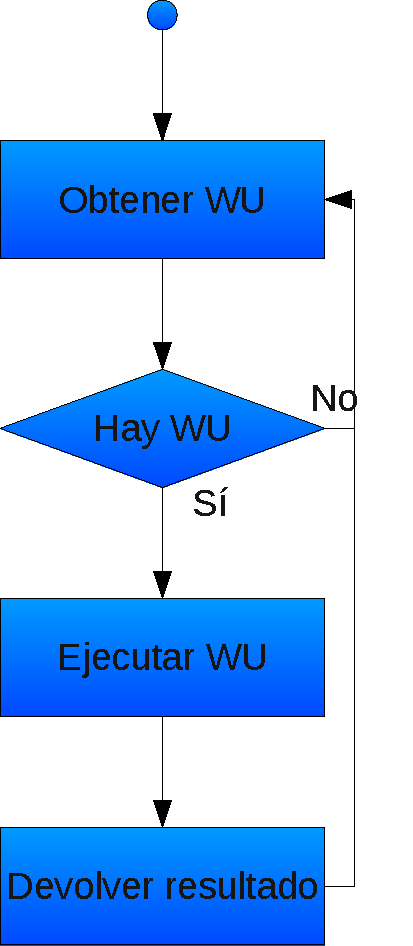
\includegraphics[width=0.26\textwidth]{images/proc_cont.pdf}
	\caption{Proceso de ejecución de un controlador}\label{fig:cont_proc_ejec}
\end{figure}

Durante el proceso de obtención de una WU, el agente comprueba si esta es valida para el algoritmo indicado. Para ello utiliza el siguiente código:

\begin{lstlisting}[language=c]
if(algorithm == "md4" || 
  algorithm == "md4_fast" || 
  algorithm == "md5" ||
  algorithm == "md5crypt" ||
  algorithm == "ntlm")
{
  hashlen = 16;
}
else if(algorithm == "sha1")
  hashlen = 20;
else        
  ThrowCustomError("Unknown hash function");
                
if(algorithm != "md5crypt" && hashlen*2 != text.length())
  ThrowError("Invalid hash length");

//Sanity check
if(hashlen > 256)
  ThrowError("Hash length too long");
if(text.length() == 0)
  ThrowError("Empty hash");
\end{lstlisting}

El problema del código mostrado anteriormente es que requiere forzosamente que ante la cualquier cambio de un algoritmo, o ante la creación de un algoritmo nuevo, modificar ese código. De este modo no el código no aprovecha la capacidad de abstracción de que otorga el lenguaje C++ ya que podría haberse hecho esto de un modo más elegante como se comprobará más adelante. Además, la el código mostrado anteriormente supone un problema para el mantenimiento ya que éste se encuentra en un fichero del código fuente, pero además, en otro completamente distinto también se hacen comprobaciones sobre los algoritmos por lo que hay que tener un buen conocimiento sobre la estructura interna del código y la organización de sus ficheros.

\section{Modificaciones realizadas a DHC}

Como se ha podido ver en el apartado anterior DHC es una buena aplicación, pero tiene algunos fallo que podrían resolverse para mejorar la mantenibilidad de la solución. Esto ofrecería una esperanza de vida mayor al programa y lo convertiría en una herramienta mucho más útil a corto y largo plazo.

Por los motivos anteriores se ha decidido realizar los cambios necesarios que conviertan a DHC en una herramienta más fácil de manejar, de mantener y que permita a cualquier programador añadir funcionalidades de forma sencilla sin requerir un alto grado de conocimiento del código del agente.

\subsection{Diseño de API para algoritmos de codificación}\label{sec:api_alg}

Como ya se ha comentado anteriormente, una de las mayores deficiencias de DHC, a nuestro entender, es la falta de mecanismo sencillo para incorporar nuevos algoritmos debido, principalmente, a que el código de los algoritmos se entremezcla con la funcionalidad de controlador por distintos ficheros de código fuente. Esto supone a la hora de realizar nuevos algoritmos un problema importante al encontrarse todo el código de los mismos repartido entre distintas funciones y métodos, dificultando enormemente las labores de mantenimiento y de desarrollo. Por este motivo se ha decidido implementar una API para el desarrollo de algoritmos que aprovechando todas las funcionalidades ya existentes mejore de forma sustancial las labores de mantenimiento de la aplicación y facilite el desarrollo de nuevos algoritmos.

El diseño de la API propuesta se ha basado en dos ideas:
\begin{itemize}
	\item El algoritmo como sistema de realización de una tarea específica, como pueda ser obtener el valor que generó un determinado resumen y
	
	\item El preparador que es el mecanismo de configuración de los parámetros obtenidos del controlador para poder ser utilizados por un algoritmo.
\end{itemize}

El objetivo principal de la propuesta es permitir agrupar todo el código que rige a un algoritmo de forma que facilite la modificación del mismo y, en caso necesario, crear algoritmos nuevos sin tener que realizar un gran esfuerzo.

Gracias al API propuesto, cada algoritmo será una clase que herede de la clase \emph{Algorithm}. Esta clase abstracta define las funcionalidades mínimas que debe implementar un algoritmo para poder ser utilizado por el agente. De este modo se consigue englobar en un único lugar todo lo relativo a un algoritmo.

La clase \emph{Algorithm} define los siguiente métodos obligatorios de implementar:

\begin{description}
	\item[GetName] Devuelvel el nombre del algoritmo. Este nombre se utiliza para poder identificar el algoritmo y poder seleccionarlo cuando se solicite. Para garantizar el buen funcionamiento del sistema y evitar funcionamientos extraños, este nombre debe ser único.
	
	\item[HashLength] Es el tamaño que debe tener un hash para ser considerado válido. Con esto se pretende que en caso de que el controlador nos de un hash erróneo poder hacer frente al problema.

	\item[InputLength] Tamaño de la entrada recibida por el WU. Aunque en muchos casos solo comprobando el tamaño del hash sería suficiente, hay algoritmos que pueden necesitar entradas extendidas, por lo que se necesita un doble chequeo.

	\item[ExecuteCPU] Implementa el código que se encarga de utilizar la CPU para realizar la tarea solicitada.

	\item[ExecuteGPU] Ejecuta en una GPU el algoritmo con objeto de realizar la tarea de comprobación.
	
	\item[IsGPUCapable] Indica si el algoritmo tiene soporte de GPU. De este modo el sistema sabe si puede determinar el método por el que debe realizarse el procesamiento, si por CPU o por GPU.
	
	\item[IsCPUCapable] Indica si el algoritmo soporta procesamiento utilizando CPU.
\end{description}

Cada algoritmo tendría asociado un preparador. Inicialmente se adaptaría el sistema existente para disponer del primer preparador al igual que sucederá con los algoritmos ya existentes, que también serán transformados. En la Figura 3 se puede ver a grandes rasgos cómo funcionaría este sistema.

Por otra parte se ha creado una factoría de algoritmos (la clase \emph{AlgorithmFactory}) que permite acceder de forma sencilla a los algoritmos que se encuentren registrados en el sistema. Además, esta factoría permite el registro de nuevos algoritmos de forma sencilla para facilitar la implementación de nuevas utilidades.

Para poder comprender mejor como funciona el nuevo sistema la figura~\ref{fig:algotirmo_gpu} muestra a grandes rasgos como sería el proceso. En este caso el actor es el agente que va a hacer uso de la funcionalidad ofrecida para realizar una comprobación sobre MD5.

\begin{figure}
	\centering
	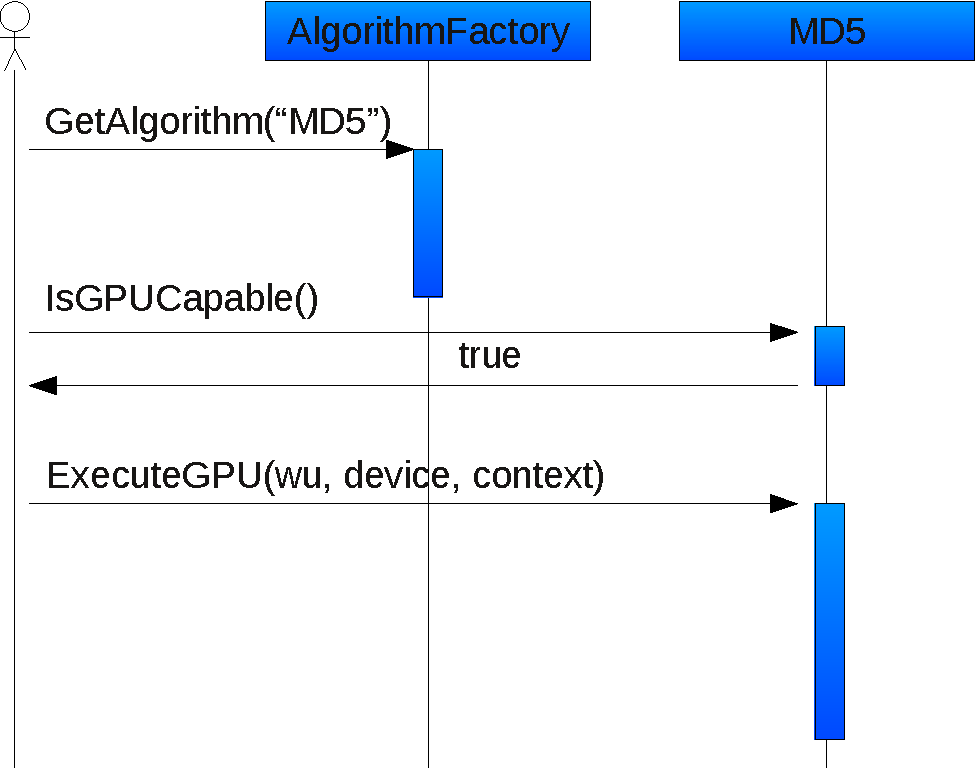
\includegraphics[width=0.7\textwidth]{images/algoritmo_gpu.pdf}
	\caption{Proceso de ejecución de un algoritmo en GPU}\label{fig:algotirmo_gpu}
\end{figure}

A la hora de implementar estas características hay que tener en cuenta que se puede hacer uso tanto de una CPU como de una GPU. Esto supone que tanto el preparador como el algoritmo deben estar capacitados para ofrecer alguna de dichas opciones y, a poder ser, ambas. Esto supone en la práctica que tanto el algoritmos implementado como el configurador pueden estar duplicados (uno especializado en CPU y otro en GPU).



\subsection{Diseño de API para la estandarización de la ejecución de algoritmos}

Una vez creado el API para algoritmos se puede comprobar que muchos algoritmos siempre siguen el mismo patrón de ejecución. Esto supone tener que repetir constantemente el mismo código en los algoritmos cuando podríamos hacer uso de la reutilización para eliminar este inconveniente. Por este motivo se planteo diseñar un sistema que permitiera estandarizar la forma que tiene un algoritmo de ejecutarse de tal modo que solo tengamos que centrarnos en lo imprescindible de cada uno de ellos.

La filosofía que se ha empleado es la misma que en el caso de los algoritmos. En este caso se ha creado la clase \emph{Executor} que se encarga de definir las funcionalidades básicas que debe implementar un mecanismo de ejecución y por otro lado se dispone de la clase \emph{ExecutorFactory} que nos facilita el acceso a los mismos.

Con este sistema se obtiene un mecanismo muy interesante para la realización de pruebas de algoritmos sin tener que modificar el resto de algoritmos y, en caso de obtener un mecanismo suficientemente bueno y que pueda ser utilizado por más algoritmos, de organizar todos los algoritmos que deban ejecutarse de igual forma para reducir la cantidad de código duplicado facilitando el mantenimiento en caso de errores.

El código original de DHC utiliza el mismo mecanismo de ejecución para todos los algoritmos implementados. Esto está muy bien hasta cierto punto ya que restringe de forma muy clara la cantidad de mecanismos que pueden implementarse en el sistema. Gracias a la nueva API se permite implementar más algoritmos, no teniendo que restringirnos necesariamente a una forma concreta de hacer las cosas o a un tipo concreto de algoritmos (hasta el momento solo hay funciones resumen).

\begin{figure}
	\centering
	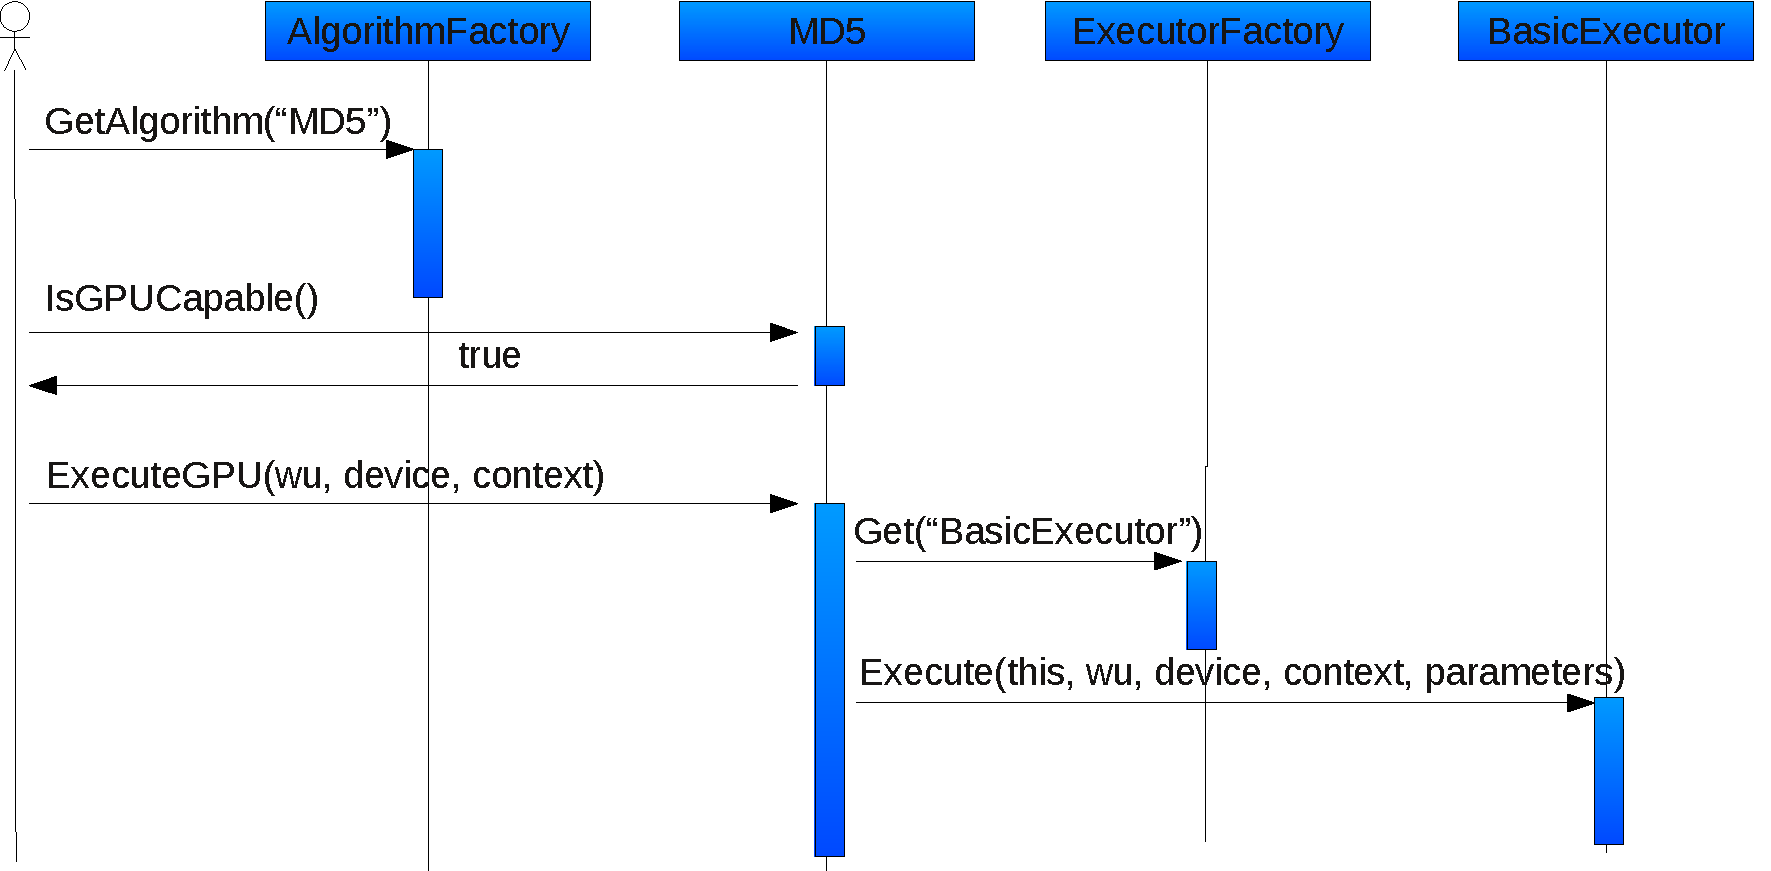
\includegraphics[width=1\textwidth]{images/executor.pdf}
	\caption{Proceso de ejecución de un algoritmo en GPU utilizando un \emph {Executor}}\label{fig:algotirmo_gpu_executor}
\end{figure}

La ejecución con este mecanismo se complica un poco más (ver figura~\ref{fig:algotirmo_gpu_executor}), pero la sobrecarga introducida por este mecanismo es despreciable en tiempo.

Una de las principales ventajas que podemos comentar sobre este sistema es que ahora un algoritmo no tiene porque estar sujeto a un único modo de hacer las cosas. Se puede detectar si hay un \emph{Executor} en concreto y si no está se pude seleccionar otro. Así, en caso de que se retire uno por cuestiones de mantenimiento o depuración el sistema podría seguir funcionando (siempre que se implemente esta forma de trabajar).

Por otra parte se permite, gracias a la arquitectura utilizada, la creación de proxys, objetos intermedios que capturan la funcionalidad expuesta para realizar operaciones de forma transparente. Por ejemplo, se podría disponer de un proxy para los algoritmos que permitiese hacer un seguimiento de las llamadas ejecutadas en caso de que el algoritmo no tuviese habilitada la generación de trazas de ejecución.

En la figura~\ref{fig:alg_ex_prox} puede verse como pueden interactuar entre sí los distintos elementos expuesto en este apartado. Como puede comprobarse, la versatilidad del nuevo sistema permite gran cantidad de configuraciones que pueden ser utilizadas siempre que sea necesario. Para comprender mejor la gráfica, los círculos representan algoritmos, las cajas son \emph{Executors} y las flechar son asociaciones de uso. Por ejemplo, \emph{MD5} usa \emph{BasicExecutor}.

\begin{figure}
	\centering
	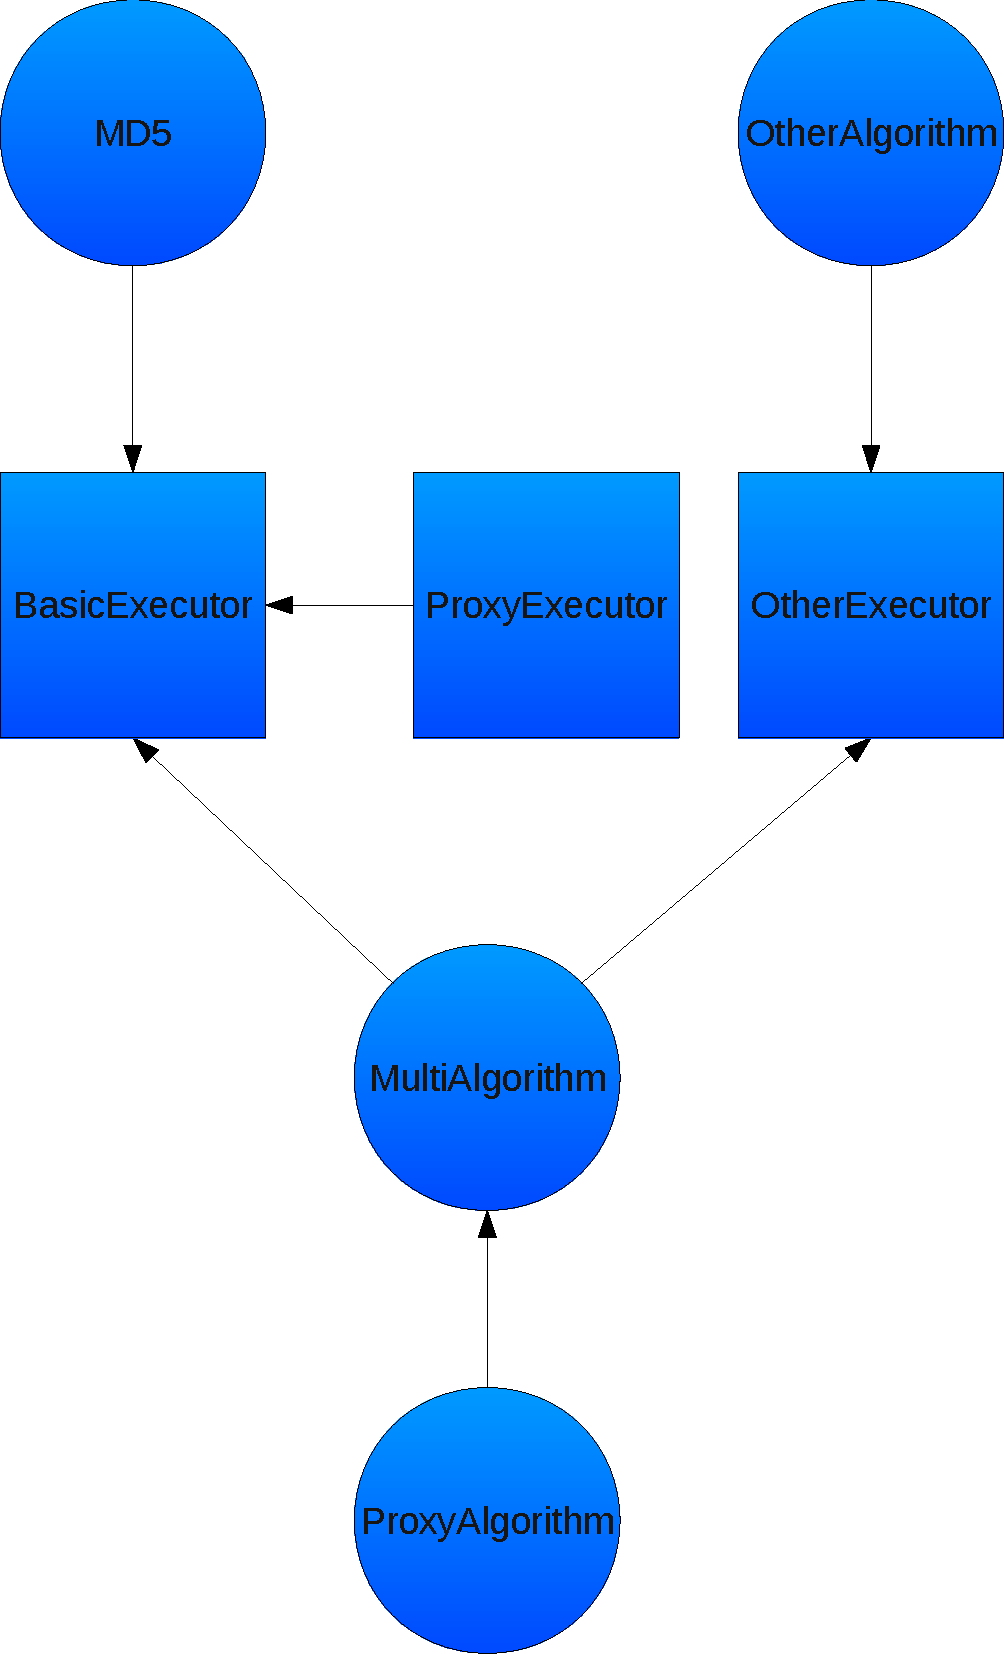
\includegraphics[width=0.4\textwidth]{images/algorithms_executors_proxys.pdf}
	\caption{Panorámica de uso de \emph{Algorithms} y \emph{Executors}}\label{fig:alg_ex_prox}
\end{figure}

\subsection{Modificaciones para la mejora de la escalabilidad}

Durante las primeras pruebas realizadas sobre DHC se notó que el tiempo de respuesta de la interfaz web podía verse seriamente comprometido si la velocidad utilizada por los agentes para solicitar tareas o devolver tareas es muy alta y si la distancia entre el agente y el controlador es grande. Este último punto se constató cuando se hicieron pruebas en las que el controlador se encontraba en un servidor en Alemania y el agente se encontraba en España. Sin duda la ralentización en este punto se debía a las latencias de la red por la espera de los asentimientos (paquetes ACK de la arquitectura IP). Estos retrasos pueden afectar de forma importante en la escalabilidad del sistema, por lo que se ha decidido realizar cambios para eliminar en la medida de lo posible estos problemas.

Cada agente de DHC se encuentra en un bucle en el que en cada iteración solicita una WU al controlador. En caso de que no haya ninguna tarea que pueda realizar el agente se procede a esperar 5 segundos. Este tiempo puede resultar insuficiente si el controlador tiene que hacer gran cantidad de cálculos o si el número de agentes es tal que saturen con peticiones al controlador (efecto DDoS). Por este motivo se ha diseñado un algoritmo que ajuste el tiempo de espera de forma dinámica para ajustarse mejor a las capacidades del controlador.

El nuevo algoritmo tiene en cuenta el tiempo que tarda el controlador en dar una respuesta al agente y si la respuesta dada contiene o no una WU. Con esto se pretende que el sistema se ajuste mejor a las condiciones ambientales del sistema.

\subsubsection{Control del tiempo con respecto al tiempo de respuesta del controlador}

Siempre que se solicitan WU a un controlador el agente mide los tiempos que tarda en recibir la respuesta. Este tiempo permite controlar si el controlador está empezando a saturarse o no. Así, en caso de que los tiempos empiecen a verse incrementados, y por tanto se considere que el controlador está saturado, se procede a incrementar el tiempo entre solicitudes. Con esto se pretende descargar al controlador de un exceso de carga distribuyéndola en el tiempo.

Por otra parte, en caso de que el tiempo disminuyese supondría justo lo contrario, la carga del controlador ha disminuido, por lo que el tiempo de espera puede empezar a reducirse poco a poco. Al realizar una disminución lenta del tiempo de espera se consigue que no se sature de repente el controlador como podría suceder si este tiempo disminuyese rápidamente.

\subsubsection{Control del tiempo con respecto a las tareas recibidas}

Aunque el ideal sería que el sistema pudiera estar constantemente funcionando, la realidad dista mucho de esto ya que es fácil que se de el caso de que no haya tareas que procesar o, que habiéndolas, éstas no sean compatibles con los agentes libres.

Teniendo lo anterior en cuenta, es fácil considerar que si en un momento dado no hay tareas, la próxima vez que consultemos al agente éste siga sin disponer de trabajos que asignar. Como este caso puede darse de forma continuada durante muchas consultas creemos que tiene sentido considerar que cada vez que se haga una petición a un controlador y éste no tenga WUs la espera hasta la siguiente vez que solicite una tarea se vea incrementado hasta un tiempo máximo. 

En caso de que el controlador empiece a ofrecer de nuevo WU a los agentes, estos empezarán a disminuir el tiempo entre solicitudes de forma paulatina hasta que vuelvan a estar estables.

La figura~\ref{fig:control_tiempo_espera} puede verse una explicación gráfica de los dos mecanismos explicados. Las variables utilizadas son:
\begin{description}
	\item[Tesp:] representa el tiempo de espera que se utilizará en caso de que se considere que el sistema no está respondiendo correctamente.
	
	\item[Tresp:] contiene el tiempo que ha tardado el controlador en devolver una respuesta al agente.
	
	\item[Tant:] es el tiempo que tardó el agente en responder en la anterior consulta.
	
	\item[MAX\_TESP:] representa el tiempo máximo que puede estar esperando antes entre consultas al controlador.
	
	\item[MIN\_TESP:] es el tiempo mínimo entre llamadas al controlador.
\end{description}

\begin{figure}
	\centering
	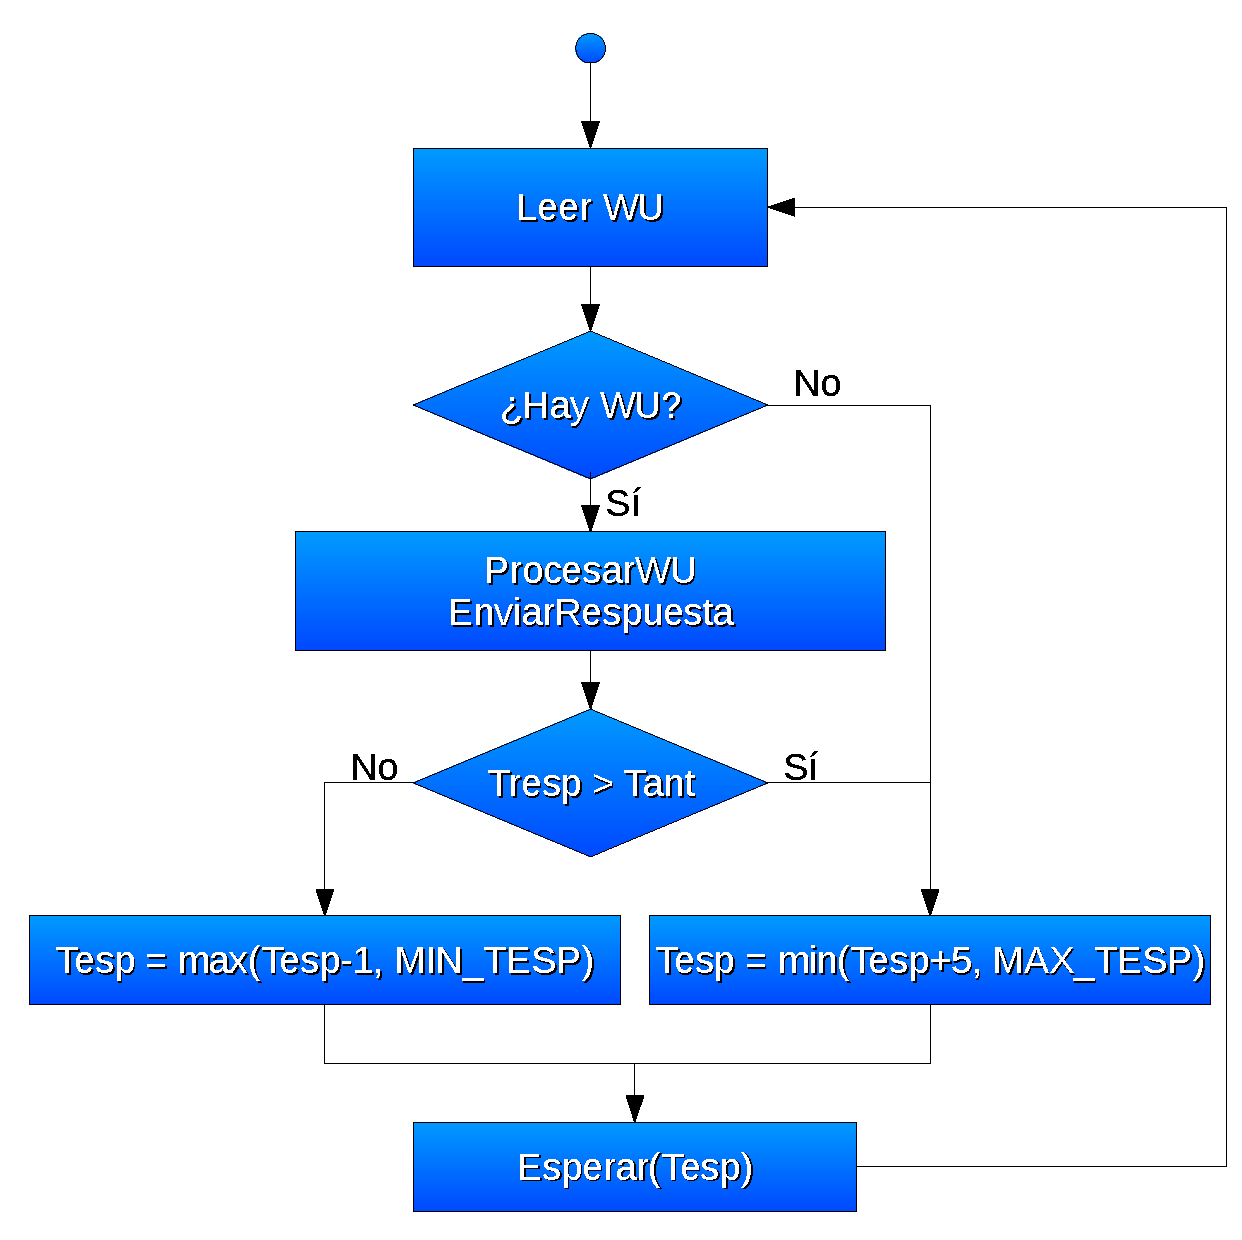
\includegraphics[width=0.7\textwidth]{images/control_tiempo_espera.pdf}
	\caption{Control del tiempo de espera en las solicitudes}\label{fig:control_tiempo_espera}
\end{figure}

\section{Diseño e implementación de un mecanismo de carga de extensiones}

Ahora que se dispone de un API que facilita la creación de algoritmos y mecanismos para ejecutar éstos, se ha diseñado un sistema que permite cargar nuevos algoritmos y \emph{Executors} que se encuentren fuera de la aplicación. Estos algoritmos y \emph{Executors} que pueden cargarse de este modo son denominados \emph{plugins}.

Para comprender mejor la idea hay que tener en cuenta que hasta este momento, si se modificaba un algoritmo al estar este dentro del programa había que generar un nuevo ejecutable con dicha modificación. Lo que se pretende es que el algoritmo no tenga que formar parte del agente y que pueda ser una unidad que se encuentre por separado.

Para poder implementar este apartado se ha desarrollado una serie de clases (figura~\ref{fig:plugins}) que van a permitir describir el contenido de un fichero que pueda ser cargado desde fuera, el contenido del mismo y añaden facilidades para poder crear instancias de las clases que defina. Las clases definidas son:

\begin{description}
	\item[PluginFacility:] clase abstracta que describe una funcionalidad que va a presentar el plugin al agente. Esta está identificada por un nombre, su versión y el tipo. Además, permite crear instancias de la funcionalidad.
	
	\item[PluginFacilityAlgorithm:] permite que el plugin pueda ofrecer a los agentes algoritmos. Esta clase implementa PluginFacility.
	
	\item[PluginFacilityExecutor:] permite que el plugin pueda ofrecer a los agentes \emph{Executors}. Esta clase implementa PluginFacility.
	
	\item[PluginFactory:] esta clase debe ser instanciada en el plugin y en ella hay que registrar todos aquellos componentes que ofrecerá el plugin al agente. Cada componente a ofrecer deberá heredad de PluginFacility. Además, esta clase proporciona información extra como el autor del plugin o el listado de \emph{facilites} que se van a exportar.
\end{description}

Además de lo anterior, los plugins deben contener una función llamda \emph{GetPluginFactory} que permitirá obtener la instancia de \emph{PluginFactory} que tiene el plugin.

\begin{figure}
	\centering
	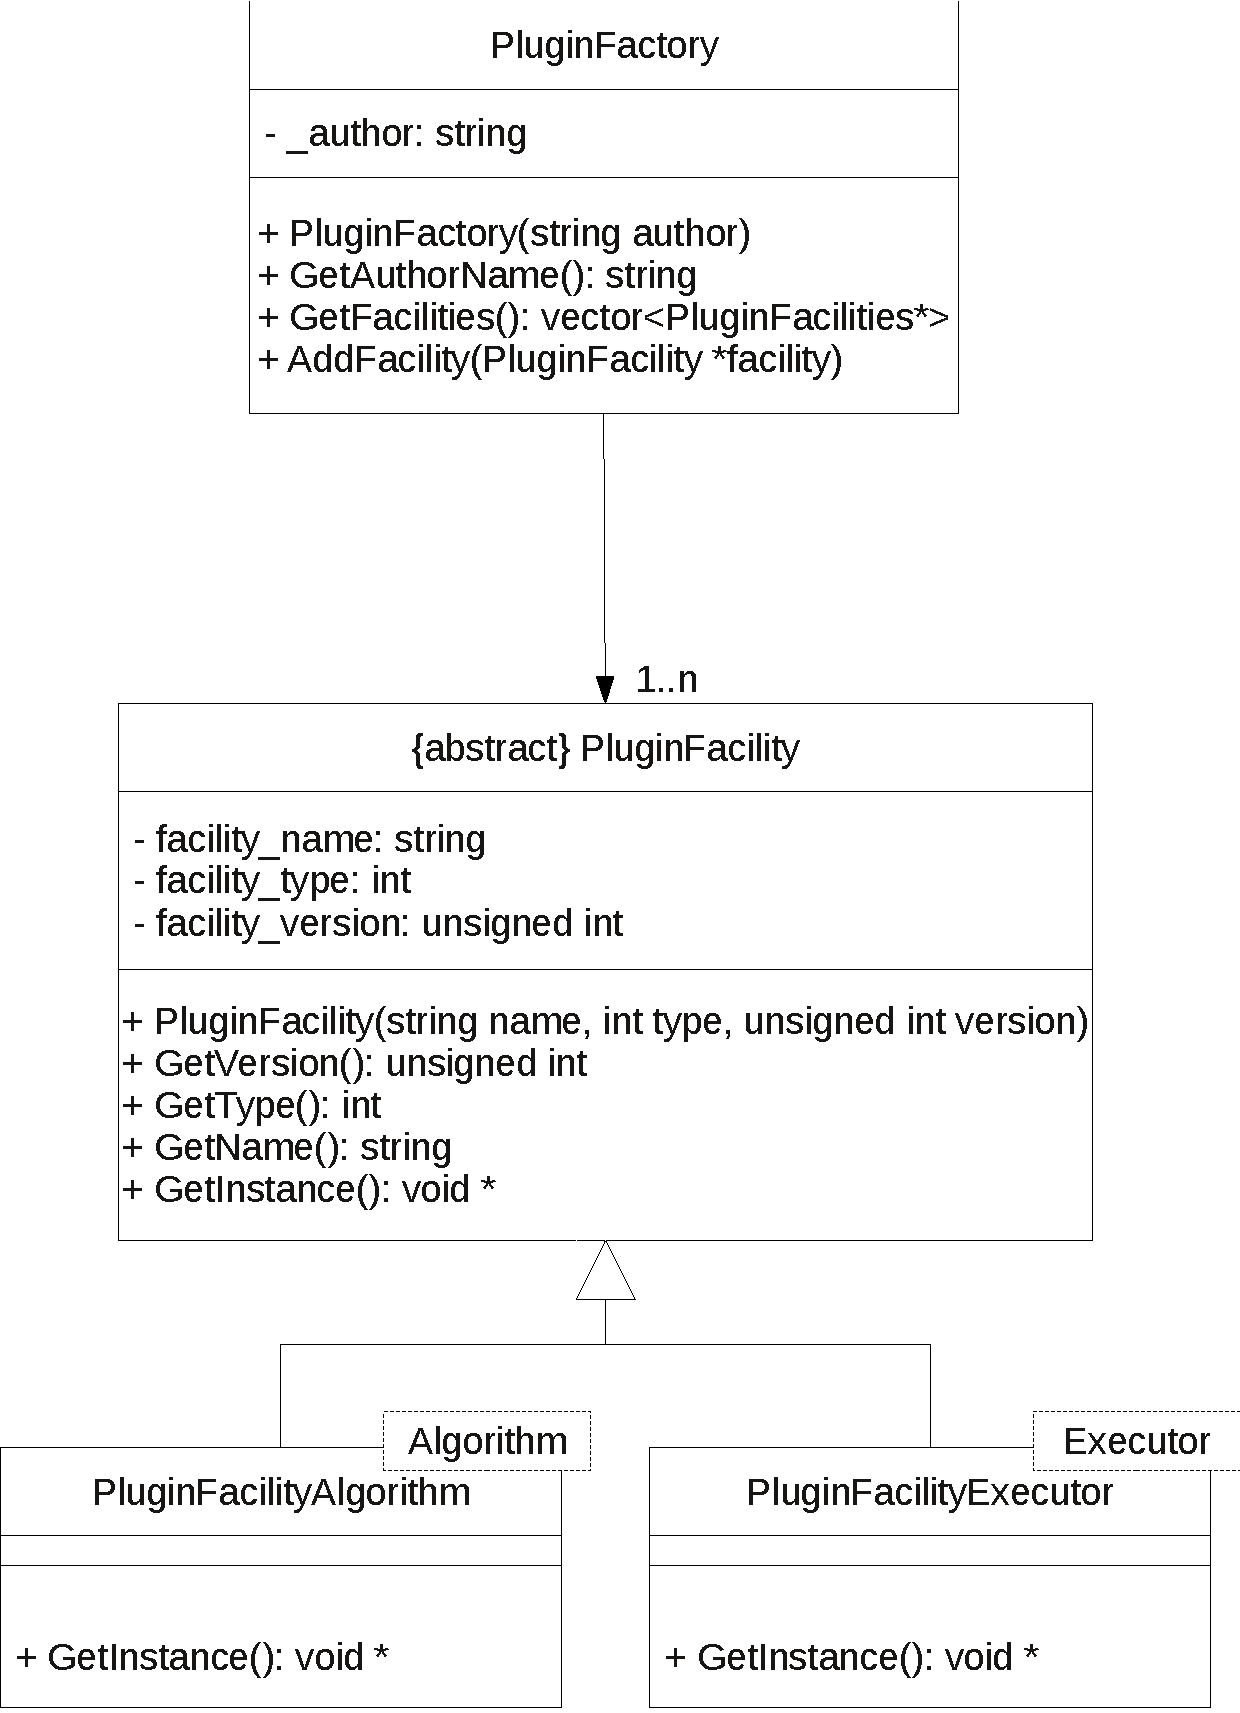
\includegraphics[width=0.7\textwidth]{images/plugins.pdf}
	\caption{Diseño del sistema de plugins}\label{fig:plugins}
\end{figure}

Como tener que memorizar todo el proceso de crear un plugin puede resultar muy complicado (intervienen muchas clases con dependencias entre ellas) se ha añadido una serie de macros de C que permiten simplificar en gran medida la creación de un plugin. Por ejemplo, para la creación del algoritmo que implementa SHA256 se ha creado una clase denominada sha256 que exportamos como algoritmo del siguiente modo:

\begin{verbatim}
BEGIN_PLUGIN("Samuel Rodriguez Sevilla")
   ADD_ALGORITHM(sha256, "sha256", 1)
END_PLUGIN()
\end{verbatim}


\section{Mejoras en la depuración}

Cuando se desarrollan aplicaciones siempre hay que tener muy encuenta que se pueden producir errores durante la ejecución. Generalmenet, el método habitual para comprobar los fallos es utilizar salidas por pantalla tratando de acotar el lugar del fallo; este sistema es poco profesional por lo que para la realización de esta práctica se ha utilizado otros mecanismos.

Para comprobar la ejecución de toda aplicación en caso de errores el mejor método es el uso de un depurador, por este motivo se ha utilizado el depurador de gnu gdb. Pero aún así no siempre es suficiente con utilizar un buen depurador, sino que tener información extra a la que éste pueda darnos puede ser de gran utilidad. Por este motivo se ha implementado un sistema de trazas para depuración que no buscan la acotación de los errores, esa información ya se encuentra en el fichero de volcado creado en los fallos graves, sino que ofrece una visión más global sobre qué está sucediendo en el código. Esta información puede ser desde cuando se entra en un método, cuando se sale de éste, salida de información varia, etc.

Para activar la salida de depuración se debe llamar a cmake del siguiente modo:
\begin{verbatim}
$ DEBUG=1 cmake .
\end{verbatim}

Así, cuando cmake esté generando el fichero de Makefile tendrá conocimiento de que debe activar la opción de depuración y de generación de salida de depuración. El primero consistema en añadir el parámetro -g durante la compilación y el segundo con -DDEBUG.

Las funciones para utilizar la salida de depuración son:

\begin{description}
	\item[DO\_ENTER(class, method)] Se encarga de anunciar cuándo se entra en un método/función. También configura automáticamente el sistema para controlar cuándo se sale del método/función para que quede constancia. Sus parámetros son cadenas que representan la clase en la que nos encontramos (class) y el método (method).
	
	\item[DO\_ERROR(str)] Muestra un error por la salida de depuración. Acepta como parámetro la salida que debe mostrar.

	\item[DO\_WARNING(str)] Advierte de una situación extraña, pero que no impide a la aplicación seguir funcionando. Acepta como parámetro la salida que debe mostrar.

	\item[DO\_MESSAGE(str)] Muestra un mensaje de usuario. Acepta como parámetro la salida que debe mostrar.

	\item[DO\_LOG(str)] Muestra un mensaje de seguimiento. Acepta como parámetro la salida que debe mostrar.
	
	\item[DO\_DEBUG(str)] Información de depuración. Es útil cuando se quiere mostrar por la salida de depuración información sobre el estado de ciertas variables. Acepta como parámetro la salida que debe mostrar.

	\item[INIT\_LOG(lvl)] Inicializa el sistema de salida de depuración. Acepta como parámetro el nivel de depuración que se va a utilizar. Este nivel puede ser:
	\begin{description}
		\item[ERROR] Es el nivel más bajo de depuración. Solo se muestran las salidas de error.
		
		\item[WARINING] Siguiente nivel de depuración. Se mostrarán las salidas de los niveles anteriores y las salidas de avisos.
		
		\item[MESSAGE] Muestra las salidas de los niveles anteriores y los mensajes del programador.
		
		\item[LOG] Mensajes de seguimiento y todos los mensajes de los niveles anteriores.

		\item[DEBUG] Mensajes de depuración junto a todos los mensajes de los niveles anteriores.
	\end{description}
\end{description}
\section{Nuevo controlador}

Además de los cambios anteriores realizados al agente también se han realizado cambios en el controlador. Concretamente se ha rehecho completamente reutilizando el código justo. El motivo de la creación de este nuevo controlador se debe, principalmente, a que se quiere disponer de un sistema bien organizado y claramente centrado en la labor de controlar las tareas.

Hasta este momento el controlador se encargaba tanto de administrar las tareas como de codificar los mecanismos necesarios de control para determinar los datos de entrada, las funciones llamadas, etc. Esto se debe principalmente a que no se ha hecho uso de ningún \emph{framework} de desarrollo web que ocultase este tipo de tareas. De este modo el controlador es una aplicación con un código que entremezcla la representación de datos, el control del flujo de ejecución y las tareas administrativas.

Por el motivo anterior se decidió crear un nuevo controlador haciendo uso del \emph{framework} CakePHP (puede encontrarse en \url{http://cakephp.org/}). Este \emph{framework} tiene las siguientes características:

\begin{itemize}
	\item Abstrae la base de datos facilitando el trabajo con los datos independientemente del motor de base de datos utilizado.
	
	\item Maneja el flujo de funcionamiento de la aplicación permitiendo de este modo que el programador se centre únicamente en la labor de desarrollo de las funcionalidades el programa.
	
	\item Tiene actualizaciones constantes que, en caso de mejoras de rendimiento o estabilidad, pueden incorporarse fácilmente a nuestro desarrollo sin necesidad de realizar cambios sobre el mismo.
	
	\item Dispone de abundante documentación con gran cantidad de ejemplo, lo que facilita su aprendizaje.
	
	\item Su uso es muy sencillo.
\end{itemize}

Por otra parte, aprovechando este cambio del controlador se ha intentado realizar algunas optimizaciones. Entre ellas podemos destacar:

\begin{itemize}
	\item Optimización de la base de datos. Para ello se estudio el uso que hace el controlador de los accesos y se comprobó que las tablas de que se utilizan para realizar las estadísticas son constantemente utilizadas y éstas nunca llegan a tener un número de elementos muy elevado (el controlador borra los datos que considera antiguos). Por este motivo se ha decidido pasar estas tablas a memoria de modo que el acceso sea más rápido. El mayor problema de esta solución es que en caso de caída del la base de datos se perderían estos valores, pero al no ser información fundamental no supone una gran preocupación.
	
	\item Agrupación de accesos a base de datos. En el antiguo controlador se podía encontrar acciones que realizaban dos o tres accesos a la base de datos para modificar un mismo elemento. Para evitar esta situación lo que se ha hecho ha sido ir acumulando los cambios a realizar y una vez que no se van a hacer más se hace la actualización de la base de datos. Esto permite ahorrar algo de tiempo y reduce la carga sobre la base de datos.
\end{itemize}

Se ha tenido en cuenta el diseño de la web a la hora de reescribir el controlador considerando que un estilo más atractivo ayudaría a una mejor experiencia de usuario.

\section{Algoritmos nuevos de seguridad implementados}

Inicialmente DHC soporta los algoritmos MD4, MD5, SHA1, NTLM y MD5 crypt. Este último es una versión de MD5 utilizada por los sistemas UNIX para almacenar las contraseñas y que se forma de la siguiente forma \$ID\$SALT\$HASH, donde ID es el identificador del algoritmo de resumen empleado (1 para MD5), SALT es una semilla aleatoria que se adjunta a la contraseña a resumir y HASH es el resultado de el resumen de la unión de la contraseña y la semilla:

$$HASH = H(SALT | PASSWD)$$

Estos algoritmos se han recodificado para que se adapten a los cambios mencionados en \ref{sec:api_alg}. Tras este cambio se ha procedido al desarrollo de nuevos algoritmos que dotan al sistema de mayor funcionalidad, especialmente si son algoritmos más modernos.

Hay que tener en cuenta que a menos que se hallen debilidades contra los algoritmos el sistema de comprobación a utilizar será siempre el de fuerza bruta. Esto supone que los algoritmos más actuales sean más costosos con respecto al tiempo necesario.

Para el desarrollo de los nuevos algoritmos se ha tenido en cuenta su uso. De este modo no se han implementado aquellos que estén en desuso por ser de poca utilidad.

\subsection{SHA-256}

Este algoritmo de resumen busca sustituir al antiguo SHA-1 ya que este se vio seriamente afectado por el tamaño de los resúmenes que generaba (de 128 bits) y por el descubrimiento de ataques controla el mismo (como se ha visto en~\ref{sub:sha1}).

Para codificar este nuevo algoritmo se ha procurado hacer uso de la experiencia previa de la aplicación, procedente del estudio de la misma, y se ha reutilizado parte del código del antiguo SHA-1. De este modo se consigue reducir el tiempo de desarrollo.

La implementación de este algoritmo se ha tomado a partir de la información ofrecida por el NIST~\cite{nist:shs} y se ha probado que funciona correctamente.




	\chapter{Resultados}

En este capítulo se presentan las pruebas realizadas sobre el proyecto y los resultados obtenidos por las mismas.

Con las pruebas realizadas se ha procurado asegurar el buen funcionamiento de los cambios introducidos durante la realización del proyecto para garantizar su utilidad.

\section{Subsistema de \emph{plugins}}

Las pruebas sobre el sistema de \emph{plugins} tratan de comprobar, por una parte, el buen funcionamiento de la carga dinámica de las extensiones, así como de las mejoras suministradas por el API de algoritmos y de \emph{executors}.

Este apartado ha sido uno de los más importantes ya que todos los cambios realizados tienen un impacto importante sobre la estructura del proyecto. De este modo se debe garantizar que tras los cambios todo el sistema sigue funcionando de forma correcta.

Los pasos seguidos para el propósito descrito ha sido el siguiente:

\begin{enumerate}
	\item Paso del algoritmo de MD4 al nuevo sistema.
	
	Con esto se pretendía probar si el mecanismo de control de algoritmos funcionaba correctamente sin influir en los resultados.
	
	Se eligió el algoritmo de MD4 a lazar entre todos los implementados en DHC.
	
	\item Paso de todos los algoritmos antiguos al nuevo sistema.
	
	Así se garantizaba el buen funcionamiento en todos los casos y se podía comprobar que no hubiese código antiguo interfiriendo en en la ejecución.
	
	\item Creación de \emph{BasicExecutor}.
	
	Este \emph{executor} implementa la lógica antigua de funcionamiento de los algoritmos. Se pretende de este modo reducir la cantidad de código duplicado y comprobar a su vez el funcionamiento de este subsistema.
	
	Como en el caso anterior el primer algoritmo en hacer uso de esta funcionalidad ha sido MD4.
	
	\item Uso de \emph{BasicExecutor} en todos los algoritmos.
	
	Con este cambio se comprueba el funcionamiento real de todos los algoritmos del sistema.
	
	\item Creación del plugin \emph{DummyPlug}.
	
	Este plugin de prueba no realiza ninguna operación dentro del sistema, pero es útil para comprobar que el subsistema de plugins es capaz de cargar correctamente los mismos.
	
	\item Transformación de los algoritmos en \emph{plugins}.
	
	Finalmente, se pasaron todos los algoritmos para que hagan uso del sistema de \emph{plugins} y así comprobar el funcionamiento real. Además, de este modo se independizan los plugins del agente.
\end{enumerate}

Para realizar las pruebas anteriores se fueron realizando los cambios paulatinamente y corrigiendo los errores que surgieron. En estos momentos se puede considerar que el subsistema de \emph{plugins}, algoritmos y \emph{executors} funciona correctamente.

\section{Controlador}

El controlador ha sufrido un rediseño importante de su aspecto que ha buscando mantener la misma funcionalidad que tenía anteriormente y a la vez ofrecer una experiencia más agradabe mejorando la presentación. Para ello se ha hecho uso de las técnicas actuales de diseño web como uso de degradados.

Los cambios realizados ha supuesto una mejora constatada tras dar a probar ambas interfaces a un grupo de personas. Este grupo se componía de 7 personas completamente ajenas al desarrollo de este proyecto y constataron la mejora del mismo.

Por otro lado, los cambios en los agentes destinados a mejorar el tiempo de respuesta del controlador han contribuido a que, en momentos de alta carga de trabajo, los tiempos de espera se reduzcan. Esto supone una mejor experiencia de usuario al eliminar posibles impaciencias por la tardanza en obtener una página del controlador. Para poder comprobar este último punto solo ha sido necesario enviar un hash al sistema para que se ponga en marcha y controlar el tiempo que tarda en devolver una página.

\section{Mantenibilidad}

La facilidad de mantener el sistema era un punto importante del proyecto por la falta de organización del mismo. Con los cambios que se han introducido se ha procurado mejorar este aspecto reduciendo el número de ficheros a cambiar para pequeños cambios.

Un ejemplo claro sería la introducción de un nuevo algoritmo, que antes suponía la modificación de al menos los siguientes ficheros:

\begin{itemize}
	\item ControllerLink.cpp
	\item ComputeThreadProc.cpp
\end{itemize}

Además, puede ser necesario el cambio de más ficheros dependiendo de cómo se haya implementado el algoritmo.

Tras la reimplentación del sistema se simplifica enormemente el número de ficheros a modificar ya que ahora solo hace falta cambiar el del propio algoritmo. Igualmente, añadir nuevas funcionalidades se simplifica enormemente ya que no hay necesidad de modificar línea alguna de código sobre el agente.

Igualmente el controlador se ha visto claramente beneficiado por el uso de CakePHP ya que, gracias al uso de una estructura ordenada en la organización de los elementos que componen al software, se puede ir directamente a la parte en la que pueda haber cualquier problema para solucionarla.

\section{Algoritmo SHA-256}

Las pruebas sobre este algoritmo han consistido, por una parte, en comprobar que los resúmenes que generaba eran correctos. Una vez confirmado este punto se ha procedido a calcular el tiempo que tarda en calcular en resumen para poder compararlo con el resto de algoritmos.

Para comprobar el tiempo que tarda se eligió una palabra de prueba con minúscula, mayúsculas, números y algunso símbolos y una longitud de 8 caracteres. Tras esto se generó su resumen SHA-1 y SHA-256. Tras medir los tiempos que tardaba el sistema en encontrar la palabra para SHA-1 y SHA-256 se pudo determinar que la implementación de este último es 1,5 veces más lenta que la primera. Esto se debe principalmente a que el nuevo algoritmo requiere más pasos para obtener el resumen.

El resultado anterior es importante de cara a la implementación de nuevos algoritmos ya que será importante tener en cuenta cuanto más complejos son y, en caso de una complejidad excesiva, si es útil implementarlo. Si la complejidad de un algoritmo resultase muy elevada podría suceder que el tiempo que tardase en devolver un resultado fuera demasiado elevado. Esto significa que es importante comprobar con las ecuaciones mostradas en~\ref{sec:comprobacion_resumen} para determinar de forma anticipada los tiempos.
	\chapter{Conclusiones}

EL proyecto ha terminado existosamente tras haber realizado toda una serie de actividades que han permitido organizar y realizar el trabajo deseado. Estas actividades fueron planteadas cuando se inicio el proyecto y garantizan la buena organización del proyecto.

A continuación puede verse las actividades realizadas ordenadas según se realizaron:

\begin{itemize}
	\item Búsqueda de soluciones existentes.

		El primer paso que se realizó fue buscar si existía alguna herramienta que, siendo sofwate libre, permitiese realizar la evaluación de contraseñas utilizando tarjetas gráficas. Solo se encontró una, DHC.

	\item Estudio de la solución elegida.

		Disponiendo de una herramienta, se procedió a estudiar el código fuente de ésta para poder determinar como añadir nuevas funciones resumen y como extender las funcionalidades que éste ya tenía.

		Desgraciadamente, la documentación que tenía DHC abarcaba principalmente el proceso de compilación y ejecución, pero no detallaba cómo funcionaba por dentro por lo que se tuvo que hacer un gran esfuerzo en su estudio.

	\item Determinar las mejoras a realizar.

		Conociendo el código se podía empezar a proponer mejoras sobre el mismo. Las mejoras debían en todo momento garantizar que la herramienta se adapte completamente a los requisitos propuestos (facilidad de ampliación, fácilidad de mantenimiento, agilidad de uso, etc.).

		Las mejoras propuestas para DHC ha sido el núcleo de este proyecto y que ya se han visto anteriormente.

	\item Llevar a cabo las mejoras propuestas.

		A lo largo del capítulo~\ref{cap:mejoras} se ha podido ver el desarrollo de las mejoras propuestas, en qué han consistido y cómo se han llevado a cabo.

	\item Pruebas de aceptación.

		Para garantizar el buen funcionamiento de las modificaciones realizadas se ha tenido que comprobar que los resultados generados fueran los correctos
\end{itemize}




Tras la finalización del proyecto, y teniendo en cuenta los resultados, podemos concluir que todas las modificaciones aportadas han permitido mejorar sustancialmente la herramienta, pudiendo destacarse:

\begin{itemize}
	\item La mejora en la mantenibilidad puede considerarse muy importante tras haberse simplificado de forma importante los puntos más críticos de la herramienta. Esto supone mayor facilidad para realizar cambios en caso de errores o de tener que introducir nuevas mejoras.
	
	\item Cuando se tiene un código que hace un uso intensivo de sentencias \emph{if} anidadas este puede, en ciertos casos, ser sustituido por mecanismos de herencia. En el caso concreto del proyecto, esto ha permitido incorporar todo el sistema de algoritmos en sustitución de un mecanismo estático y complicado de modificar.
	
	\item El subsistema de \emph{plugins} permite simplificar el código del agente, separando la funcionalidad de control del mismo de las tareas más específicas que se le soliciten. De este modo DHC se convierte en una herramienta más versátil a la que se le puede dotar de nuevas funcionalidades para las cuales no había sido diseñado inicialmente.
	
	\item El uso del CakePHP ha permitido simplificar el código del controlador gracias al uso de las herramientas que éste nos ofrece. Además, esto facilita enormemente el realizar cambios sobre la interfaz y mantener una mayor organización código.
	
	\item El uso de \emph{frameworks} MVC facilita en gran medida el desarrollo de aplicaciones web al eliminar la necesidad de preocuparse por detalles de bajo nivel como puedan ser el acceso a base de datos.

	\item El nuevo diseño creado para DHC lo convierte en un sistema más atractivo, lo que anima a que sea utilizado. Este punto es importante ya que generalmente la gente se siente más agusto con aquello que encuentra agradable frente a soluciones que puedan ser más completas.
	%explicar este punto bien en la presentación
	
	\item Tras el estudio y el uso de la herramienta se puede concluir que es muy importante la calidad de las contraseñas utilizadas ya que en su fortaleza depende una parte importante de la seguridad de muchas instituciones. Igualmente, el tipo de función resumen es también importante ya que las debilidades que ésta pueda tener puede afectar enormemente a la integridad de los datos.
		
	\item Las herramientas de control de versiones simplifican enormemente la gestión del código de los proyectos ya que eliminan la necesidad de mantener las versiones manualmente. Además, al funcionar este tipo de herramientas en red permite disponer del código en cualquier parte eliminando la necesidad de tener que recordar el llevar una copia encima. Por otra parte, también facilitan las tareas de vuelta atrás en el tiempo en caso de fallos graves, de este modo en caso de cometer un error se puede ir fácilmente a una versión anterior para deshacer los cambios.
\end{itemize}

Finalmente cabe concluir que tras el desarrollo de este proyecto se ha podido comprobar las dificultades que entraña el mantenimiento de herramientas con una escasa documentación.
	\chapter{Trabajos futuros}\label{cap6}

Tras terminar el proyecto hay muchas mejoras que han quedado pendientes o sería deseable poder añadir. A continuación puede verse una lista de aquellas elementos que se han considerado más importante de cara a la continuidad del proyecto:

\begin{description}
	\item[Carga de algoritmos desde el controlador] Esta extensión permitiría centralizar la administración de los algoritmos en el controlador de modo que no haga falta tener que entrar de forma remota en cada uno de los agentes para añadir nuevas funcionalidades. Esto facilitaría la administración del sistema al evitar tener que acceder a cada agente para instalar las extensiones.

	\item[Mejorar las comunicaciones entre agentes y controlador] Hasta este momento las comunicaciones entre agente y controlador hacen uso de un protocolo un poco pobre en lo que a características se refiere lo que supone también una restricción a la hora de hacer ampliaciones. La mejora propuesta busca ampliar este protocolo para que la variedad de funciones que pueda tener el agente sea mucho mayor.

	\item[Crear nuevos algoritmos de comprobación de hashes] En la actualidad hay una gran cantidad de algoritmos de resumen que pueden ser portados a  DHC y sería interesante disponer de ellos.
	
	\item[Implementar nuevos protocolos de seguridad] DHC no tiene porque restringirse solo a funciones resumen y menos cuando no son el único mecanismo de cifrado que hay en la actualidad.

	\item[Control de cambios sobre el sistema de ficheros] Esta característica puede utilizarse para determinar cuando un plugin ha cambiado y volverlo a cargar sin tener que reiniciar el agente. De este modo el rendimiento de la aplicación mejoraría al no tener que parar casi nunca.
\end{description}

	\appendix

	\chapter{Presupuesto}

A continuación se va a presentar el presupuesto requerido para llevar a cabo del proyecto.

La duración total del proyecto ha sido de 11 meses, teniendo en cuenta que la dedicación que se ha aplicado ha sido de aproximadamente 13,2 horas semanales (un tercio de las 40 horas semanales).

\section{Desglose de actividades del proyecto}

Para calcular el total de horas del proyecto se ha tenido en cuenta todas las actividades realizadas en el mismo. En el cuadro~\ref{tab:des_horas} puede apreciarse el trabajo que ha ido desde el estudio de la solución previa, el análisis de los posibles cambios a realizar, el diseño de las modificaciones realizadas o la instalación del sistema de pruebas (la máquina Tesla).

\begin{table}
	\centering
	
	\begin{tabular}{|l|r|}
		\hline
		Actividad & Horas \\
		\hline
		Estudio DHC & 80 h \\
		\hline
		Anásis y diseño & 70 h \\
		\hline
		Implementación & 280 h \\
		\hline
		Pruebas & 40 h \\
		\hline
		Instalación sistema & 5 h \\
		\hline
		Documentación & 100 h \\
		\hline
	\end{tabular}
	\caption{Desglose de horas por actividad}\label{tab:des_horas}
\end{table}

\section{Gasto en personal imputable al proyecto}

Para ajustar el precio por hora del programador se ha hecho una búsqueda entre las ofertas de trabajo que se encuentran actualmente en internet. Se ha tomado como muestra aquellas en las que se busca profesionales con experiencia donde el sueldo ronda los 36.000\euro/año.

El coste total por personal es de 9.200\euro como puede apreciarse en el cuadro~\ref{tab:des_prec_horas}.

\begin{table}
	\centering
	
	\begin{tabular}{|l|r|r|r|}
		\hline
		Cargo & Horas & Coste/Hora & Total \\
		\hline
		Analista & 150 h & 16,00\euro/hora & 2.400,00\euro\\
		\hline
		Programador & 280 h & 16,00\euro/hora & 4.480,00\euro\\
		\hline
		Responsable documentación & 100h h & 16,00\euro/hora & 1.600,00\euro\\
		\hline
		Responsable pruebas & 40 h & 16,00\euro/hora & 640,00\euro\\
		\hline
		Técnico instalación & 5 h & 16,00\euro/hora & 80,00\euro\\
		\hline
		\hline
		Total & 575 h & \multicolumn{2}{|r|}{9.200,00\euro} \\
		\hline
	\end{tabular}
	\caption{Desglose de horas por actividad}\label{tab:des_prec_horas}
\end{table}


\section{Servicios subcontratados}

En el cuadro~\ref{tab:serv_subcont} puede apreciarse el coste de los servicios que se han subcontratado.

\begin{table}
	\centering
	
	\begin{tabular}{|l|r|r|r|}
		\hline
		Servicio & Precio mes & Meses & Total\\
		\hline
		Servidor privado virtual & 16,99\euro/mes & 11 & 186,89\euro\\
		\hline
		\hline
		\multicolumn{3}{|l|}{Total} & 186,89\euro\\
		\hline
	\end{tabular}
	\caption{Coste de los servicios subcontratados}\label{tab:serv_subcont}
\end{table}

\section{Recursos materiales empleados}

Durante la realización de este proyecto se ha hecho uso de una gran cantidad de software. Al haber sido software libre y gratuito el coste repercutido a un posible cliente es de 0\euro y no hace falta amortizarlo lo que puede ser considerado una ventaja importante frente a otros sistemas que pueden encarecer significativamente el producto.

Por lo anterior, solo es necesario repercutir el coste de los dispositivos materiales empleados, como puede verse en el cuadro~\ref{tab:re_mat}.

\begin{table}
	\centering
	
	\begin{tabular}{|l|r|r|}
		\hline
		Recurso & Cantidad & Coste total \\
		\hline
		Ordenador personal & 2 & 3.000,00\euro \\
		\hline
		Tesla T1070 & 1 & 7.082,00\euro \\
		\hline
		Servidor Tesla & 1 & 2.528,00\euro\\
		\hline
		\hline
		\multicolumn{2}{|l|}{Total} & 12.610,00\euro\\
		\hline
	\end{tabular}
	\caption{Coste de los recursos materiales empleados}\label{tab:re_mat}
\end{table}

\section{Gastos indirectos}

Se debe tener en cuenta el coste de todos aquellos elementos que si bien no repercuten directamente sobre el proyecto suponen un gasto constante durante la vida de éste.

\begin{table}
	\centering
	
	\begin{tabular}{|l|r|r|}
		\hline
		Descripción & Coste \\
		\hline
		Conexión a internet & 143,50\euro \\
		\hline
		Llamadas telefónicas & 143,50\euro \\
		\hline
		Material de oficina & 10,00\euro\\
		\hline
		Alquiler local & 3.953,13\euro\\
		\hline
		Electricidad & 74,75\euro\\
		\hline
		Servicio de limpieza & 3593,75\euro\\
		
		\hline
		\hline
		Total & 7.918,63\euro\\
		\hline
	\end{tabular}
	\caption{Costes indirectos}\label{tab:cost_indi}
\end{table}

El precio de la conexión a internet y de la telefonía se ha calculado a partir de las facturas obtenidas de unos 40\euro/mes cada una. Considerando que un mes tiene 4 semanas a 40 horas laborables el precio por hora es de 0,25\euro/hora. Este valor se multiplica por el total de horas empleadas para realizar el proyecto.

El material de oficina comprende folios, cuadernos e instrumental para escribir. Apenas se ha gastado material de este tipo (un cuaderno, algunos folios y un bolígrafo) por lo que su valor es bajo.

El alquiler de locales en Leganés están sobre los 1.100\euro/mes de media (obtenido a partir de una revisión de \url{www.idealista.com}). Estos locales solo pueden amortizarse durante la actividad económica del mismo (40h/semana). Esto supone un coste por hora de 6,875\euro/hora.

Se ha supuesto un gasto en electricidad de unos 20\euro/mes. Esto supone un coste por hora de 0,13\euro/hora.

La limpieza del local puede rondar en torno a los 1.000\euro/mes. Se ha considerado que la subcontratación del servicio de limpieza puede rondar los 25\euro/hora y no sería necesario más de 2 horas al día durante cada día de la semana (unos 20 días al mes). Esto supone un coste distribuido por horas de 6,25\euro/hora.

En el cuadro~\ref{tab:cost_indi} hay un resumen de los gastos indirectos del proyecto.

\section{Resumen del presupuesto}

\begin{table}
	\centering
	
	\begin{tabular}{|l|r|}
		\hline
		Descripción  & Coste  \\
		\hline
		Personal     & 9.200,00\euro \\
		\hline
		Subcontratas & 186,89\euro \\
		\hline
		Material     & 12.610.00\euro\\
		\hline
		Indirectos   & 7.918,63\euro\\
		\hline
		\hline
		Total        & 29.915,52\euro\\
		\hline
	\end{tabular}
	\caption{Resumen de los gastos del proyecto}\label{tab:resu_gastos}
\end{table}

Con todos los datos juntos (ver cuadro~\ref{tab:resu_gastos}) precedemos a calcular el precio de venta de la solución desarrollada.

Lo primero de todo es que pueden darse imprevistos a lo largo del desarrollo, como roturas de material, enfermedad del personal, etc. Por este motivo se aplica un margen del 10\% sobre el precio para compensar estos posibles imprevistos: 2.991,55\euro.

$$
\mbox{Coste Total} + \mbox{Margen de imprevistos} = \mbox{32.907,07\euro}
$$

El margen de beneficio a aplicar es del 25\% sobre el precio con imprevistos: 8.226,77\euro.

$$
	\mbox{Precio Final} = \mbox{Precio con Imprevistos} + \mbox{Beneficio} = \mbox{41.133,84\euro}
$$

El precio final de la solución, contando el 18\% de I.V.A., es: {\large \textbf{48.537,93\euro}}.
	\chapter{Entorno de desarrollo}\label{chap:entorno}

Para el desarrollo del proyecto se ha hecho uso de una gran cantidad de herramientas y tecnologías que es importante ver para poder comprender mejor el modo de desarrollo.

\section{CMake}

CMake es una herramienta para la construcción de ficheros Makefile. El mayor inconveniente que hay a la hora de utilizar ficheros Makefile es que es complicado mantenerlos y aún más crear versiones para diferentes sistemas operativos. Este último punto se debe a que puede variar sutilmente algunas de las reglas de para crear el fichero y que dependiendo del sistema operativo se puedan necesitar unas u otras librerías. Además, utilizando ficheros Makefile es complicado realizar comprobaciones sobre el sistema, com puedan ser comprobar si está o no instalada una biblioteca en concreto.

Existen varias soluciones para la generación de ficheros Makefile, entre ellas destaca GNU Autotools. Ésta es probablemente una de las herramientas más famosas en el mundo del software libre por ser la que se utiliza dentro del proyecto GNU. Desgraciadamente Autotools es una herramienta complicada de utilizar lo que nos hizo decantarnos por CMake.

CMake utiliza una sintaxis sencilla para definir las reglas de comprobación, asignación de dependencias y cualquier cosa que tenga que ver con el proceso de generación del proyecto.

Para instalar cmake en el sistema se ejecutará el siguiente comando:

\begin{verbatim}
$ sudo apt-get install cmake
\end{verbatim}

\section{Git}

Una parte muy importante de todo proyecto es la gestión de los ficheros que se están utilizando. En el caso de un proyecto software el control de los cambios es fundamental para evitar problemas.

Git es un sistema de control de versiones desarrollador por Linus Torvalds para el núcleo Linux. Sus principales características son:

\begin{itemize}
	\item Es un sistema distribuido, lo que evita la necesidad de disponer siempre de un servidor central al que enviar los cambios, como sucede con otros sistemas como CVS o Subversion.
	
	\item Facilita la creación de ramas (\emph{branch}) de desarrollo y la fusión de éstas (\emph{merge}) cuando es necesario de forma rápida y sencilla.
	
	\item Facilita disponer de copias de seguridad distribuyéndolas entre varios equipos, al menos en el uso que se ha dado para este proyecto final de carrera.
\end{itemize}

Para poder utilizar git solo hace falta instalarlo ejecutando el siguiente comando:

\begin{verbatim}
$ sudo apt-get install git-core
\end{verbatim}

Durante el desarrollo del proyecto se ha utilizado varias ramas para controlar las distintas partes. Concretamente se ha utilizado:

\begin{description}
	\item[master] Mantiene el código que ha se ha comprobado que funciona correctamente. No se puede incorporar nada a esta rama directamente, sino que hay que desarrollar primero en otra rama, comprobar correcto funcionamiento de los cambios y luego se realiza la mezcla de los cambios con \emph{master}s.
	
	\item[ldopen] En esta rama se realizaron los cambios para soportar plugins. La nomenclatura de ldopen proviene de la llamada a sistema utilizada para poder desarrollar esta funcionalidad.
	
	\item[nuevaweb] Aquí se encuentra todo el código de pruebas del nuevo controlador desarrollado así como cambios sobre los agentes para soportar la nueva arquitectura.
	
	\item[fixcompiling] Cambios realizados para que la compilación en el sistema operativo Mac OS X funcionara correctamente.
\end{description}

\section{Apache}

Para poder hacer uso del controlador es necesario disponer de un servidor web con soporte de PHP. En este caso se ha utilizado el servidor web Apache en su versión 2 por ser el más popular, disponer de una abundante documentación y ser software libre.

Cualquier distribución de GNU/Linux puede instalar este servidor web con unos pocos \emph{clicks} de ratón o en su defecto un único comando. en el caso de las distribuciones basadas en Debian solo hace falta ejecutar el siguiente comando:

\begin{verbatim}
$ sudo apt-get install apache2
\end{verbatim}

\section{Redmine}

Redmine es un gestor de proyectos realizado en Ruby on Rails. Permite la asignación de tareas, calendarios, documentación y otras muchas funcionalidades más a través de plugins. Como la mayoría de las herramientas utilizadas es software libre.

Esta herramienta ha sido de utilidad para poder controlar los problemas que han ido surgiendo y que no quedaran pendientes.

La instalación de redmine es probablemente de las más complicadas de todas las herramientas utilizadas en este proyecto. Para instalar esta herramienta se ha tenido que seguir los siguientes pasos:

\begin{itemize}
	 \item Instalación de ruby, rails y rake:
	 \begin{verbatim}
	 $ sudo apt-get install ruby rails rake
	 \end{verbatim}
	 
	 \item Instalación del módulo \emph{passenger} para apache\footnote{Passenger dispone de paquetes para algunas distribuciones. Por desgracia, la distribución que utilizaba el servidor de Redmine no disponía de dichos paquetes}:
	 \begin{verbatim}
	 $ sudo gem install passenger
	 $ sudo passenger-install-apache2-module
	 \end{verbatim}
\end{itemize}

\section{CUDA}

Como no, se ha hecho uso de las herramientas de NVIDIA para compilar el proyecto. El \emph{framework} CUDA trae las bibliotecas básicas necesarias para poder comunicarse con la tarjeta gráfica y las herramientas de compilación.

Para poder utilizar CUDA hay que instalar previamente los controladores de la tarjeta gráfica adecuados ya que los controladores que vienen por defecto solo permiten funciones gráficas.

Para desarrollar el proyecto se ha hecho uso de la versión 2.3 de CUDA que puede encontrarse en \url{http://developer.nvidia.com/object/cuda_3_2_downloads.html}. Desde esta página se pueden descargar tanto los controladores para el sistema operativo como las herramientas necesarias para desarrollar en CUDA.

Es importante comprobar antes de utilizar CUDA si la tarjeta gráfica que tiene el equipo es compatible.

Para instalar CUDA en linux se necesita instalar primero el controlador de la tarjeta gráfica. Este controlador requiere las cabeceras del núcleo Linux para poder compilarse. Por este motivo hay que asegurarse de que ya se encuentre instaladas y en caso contrario se pueden instalar con el siguiente comando:

\begin{verbatim}
$ sudo apt-get install linux-headers-generic
\end{verbatim}

Por desgracia no se ofrecen paquetes adaptados a cada distribución por lo que hay que utilizar el instalador que ofrece NVIDIA:

\begin{verbatim}
$ wget http://developer.download.nvidia.com/compute/cuda/
3_2_prod/drivers/devdriver_3.2_linux_32_260.19.26.run
$ sudo sh ./devdriver_3.2_linux_32_260.19.26.run
\end{verbatim}

Tras este paso solo hay que seguir las indicaciones del instalador.

Hay ocasiones en las que el instalador de los controladores de NVIDIA fallan y no crean los dispositivos necesarios en \emph{/dev}, por lo que hay que crearlos a mano. Para ello se puede utilizar las siguiente llamadas en línea de comando:

\begin{verbatim}
$ for i in $(seq 0 9); do sudo mknod /dev/nvidia${i} c 195 ${i}; done
$ sudo mknod /dev/nvidiactl c 195 255
\end{verbatim}

Una vez instalado el controlador de CUDA se puede proceder a instalar las herramientas. Éstas utilizan su propio instalador, pero está adaptado a distintas distribuciones, por lo que hay que elegir el más adecuado:

\begin{verbatim}
$ wget http://developer.download.nvidia.com/compute/cuda/
3_2_prod/toolkit/cudatoolkit_3.2.16_linux_64_ubuntu10.04.run
$ sudo sh ./cudatoolkit_3.2.16_linux_64_ubuntu10.04.run
\end{verbatim}

Es recomendable instalar las herramientas en los directorios que nos indique como predeterminados (generalmente \emph{/usr/local/cuda}).

\section{GNU G++}

El compilador de GNU es probablemente uno de los más utilizados hoy día en el mundo del software libre. Este compilador dispone de herramientas para compilar una gran cantidad de lenguajes distintos como C, C++, Objective-C, Pascal y muchos más. Es el compilador que traen todas las distribuciones GNU/Linux en la actualidad y hasta sistemas operativos como Mac OS X lo utilizan.

La mayor parte del código empleado en el proyecto está escrito en C++ por lo que se ha necesitado hacer uso del compilador de C++ que de GNU, principalmente por ser el más sencillo de instalar.

Para asegurarnos que al instalar el compilador GNU G++ se instalen todas las dependencias que necesitamos podemos ejecutar la siguiente orden:

\begin{verbatim}
$ sudo apt-get install build-essential g++
\end{verbatim}

El paquete \emph{build-essential} se encarga de instalar todas las herramientas y bibliotecas de compilación básicas. Luego le indicamos que se asegure de instalar g++.

\section{NASM}

NASM es un ensamblador multiplataforma que se necesita para poder generar la versión de CPU de MD5. Es importante asegurarse de utilizar la última versión de la herramienta ya que, por ejemplo, la versión que trae Mac OS X no está actualizada y no permite realizar compilaciones de 64 bits.

Para instalarlo solo hay que ejecutar:

\begin{verbatim}
$ sudo apt-get install nasm
\end{verbatim}

\section{PHP}

PHP es un lenguaje de programación web muy extendido gracias a que es gratuito y libre. Tiene una sintaxis sencilla fuertemente basada en C y es muy fácil de aprender.

Es muy habitual hablar de instalaciones LAMP, que son aquellas que hacen uso de Linux, Apache, MySQL y PHP y que son ampliamente utilizadas en internet por gran número de servicios de alojamiento por su bajo coste y facilidad de instalación y configuración.

Al ser un lenguaje muy extendido se ha utilizado para la creación del nuevo controlador de DHC. El anterior controlador también hacía uso de PHP pero cuando se planteó crear uno nuevo se barajaron soluciones basadas en Ruby y Groovy. Estas soluciones fueron descartadas por ser algo más complicadas de configurar. Para ser más precisos, Ruby requiere que se instalen módulos especiales para Apache y hay que revisar muy bien la configuración. En el caso de Groovy se necesita un servidor Apache Tomcat basado en java que puede suponer una gran sobrecarga para el sistema.

Para instalar PHP e integrar éste con Apache solo hace falta ejecutar el siguiente comando en cualquier distribución basada en Debian:

\begin{verbatim}
$ sudo apt-get install php5
\end{verbatim}

\section{CakePHP}

CakePHP es un \emph{framework} de desarrollo web que hace uso del lenguaje de programación PHP y el patrón arquitectónico MVC. Con CakePHP se pueden hacer aplicaciones fácilmente sin tener que preocuparse de cosas como el acceso a base de datos o el control de flujo a través de la aplicación.

Gracias al uso de CakePHP se ha podido centrar la atención del controlador más en las tareas propias del mismo. De este modo ahora no hay que preocuparse de como hacer el acceso a la base de datos o incluso el tipo de base de datos que se está utilizando.

Para utilizar CakePHP solo hace falta descargarlo y descromprimirlo en un directorio. Éste ya dispone de una estructura básica de directorios para utilizar directamente en un proyecto. Para este proyecto los directorios más importantes son:

\begin{description}
	\item[app/controllers] Almacena los controladores de la aplicación. Estos controladores se encargan de la lógica de negocio.
	
	\item[app/views] Representan las salidas que producirá la aplicación.
	
	\item[app/models] Describe la estructura de la base de datos (las tablas y sus relaciones).

	\item[app/config] Tiene la configuración del motor de base de datos que hay que utilizar y la configuración de la misma. Por otra parte se ha almacenado aquí el script para generar las tablas en esta base de datos.
\end{description}

\section{MySQL}

MySQL es uno de los motores de base de datos libres más extendidos de internet. La principal razón de esto es que es fácil de administrar y que históricamente siempre ha sido una base de datos muy rápida, lo que suponía una ventaja para las aplicaciones web con una alta carga de peticiones.

El controlador de DHC hace uso de bases de datos para almacenar la información de las tareas que se están ejecutando y las estadísticas de las mismas.

Su instalación es tan sencilla como ejecutar:

\begin{verbatim}
$ sudo apt-get install mysql-server
\end{verbatim}

\section{Gimp}

Gimp es una herramienta de retoque fotográfico de una gran calidad y que desde hace muchos años se la considera el Photoshop del software libre.

Para las imágenes utilizadas en la web se ha utilizado Gimp por ser una herramienta potente y relativamente sencilla de utilizar.

Para su instalación se ha utilizado:

\begin{verbatim}
$ sudo apt-get intall gimp
\end{verbatim}

\section{\LaTeX}

Es una de las herramientas más extendidas para la creación de textos científicos. \LaTeX son un conjunto de reglas para la herramienta \TeX creada por Donald E. Knuth. Su diseño está pensado para no tener que prestar demasiada atención a detalles de presentación para centrar el esfuerzo en el contenido. Es muy parecido a lo que ahora se hace en web con HTML+CSS.

La memoria de este proyecto final de carrera ha sido escrito utilizando \LaTeX por las ventajas que ofrece frente a otros sistemas como Microsoft Word o LibreOffice. Entre estas ventajas podemos destacar que al almacenar solo ficheros de texto es más sencillo realizar un control de versiones sobre las modificaciones, lo que resulta más complicado utilizando ficheros binarios.

Para instalar el compilador de \LaTeX en el sistema hay que ejecutar:

\begin{verbatim}
$ sudo apt-get install texlive-latex-extra
\end{verbatim}

\section{GnuPlot}

GnuPlot es una herramienta para la generación de gráficas de funciones. Ha sido utilizada para la gráfica de la distribución de la paradoja del cumpleaños.

Esta herramienta es muy útil cuando se necesita hacer gráficas de datos y no se tiene un sistema muy potente ya que requiere de poca memoria. Un ejemplo de ello es cuando se tienes grandes tablas de datos en MS Office lo que hace que tarde en generar gráficas o incluso manejar los datos.

En este caso se ha creado un script de GnuPlot que ha sido integrado dentro del sistema de compilación automático de CMake para generar un PDF y poder ser incrustado en el documento \LaTeX.

Para instalar GnuPlot solo hace falta utilizar la siguiente orden en el sistema:

\begin{verbatim}
$ sudo apt-get install gnuplot
\end{verbatim}

\section{LibreOffice}

LibreOffice es una herramienta que ha nacido a partir del código de OpenOffice.org. Su creación viene motivada a que los desarrolladores de OpenOffice.org estaban a disgusto con las políticas empresariales de Oracle.

Todas los diagramas que aparecen en la memoria ha sido realizadas con la aplicación de dibujo de LibreOffice.

LibreOffice puede ser descargado desde su página web en \url{http://www.libreoffice.org/download/}.

\section{UML}

UML, siglas de \emph{Unified Modeling Language}, es un lenguaje gráfico para modelar software ampliamente utilizando en el mundo de la programación orientada a objetos.

Algunos de los diagramas expuestos en la memoria hacen uso de dicho lenguaje. Concretamente se ha hecho uso de diagramas de clases y de secuencia. El primero permite expresar de forma gráfica los elementos que formar todo, o una parte, de un programa, pero sin entrar al detalle de como deben comportarse. Los diagramas de secuencia representan un caso de funcionamiento concreto y son útiles para poder mostrar cómo actúa una parte del proyecto.

\section{Debian y Ubuntu}

Debian es una de las distribuciones de Linux más antiguas y su filosofía es utilizar sólo software libre. Una de los puntos más importantes a destacar sobre esta distribución es que está mantenida enteramente por voluntarios y que tiene uno de los mayores repositorios de aplicaciones de todas las distribuciones existentes.

Debian posee muchas distribuciones derivadas que sobre ésta añaden paquetes y/o hacen cambios de configuración. Una de estas distribuciones, y probablemente la distribución más famosa actualmente, es Ubuntu.

Para descargar Debian se puede ir a \url{http://www.debian.org/distrib/} y Ubuntu se puede obtener de \url{http://www.ubuntu.com/desktop/get-ubuntu/download}.

%\section{SLOCCount}

%SLOCCount es una herramienta para contar número de líneas de código de proyectos software. Tras una ejecución de esta herramienta sobre un directorio con software ofrece estadísticas del número de líneas total y cómo se distribuyen entre los distintos lenguajes de programación utilizados.

%Además de lo anterior, SLOCCount trata de hacer una estimación del coste del código comprobado utilizando el modelo COCOMO.

%Para poder utilizar esta herramienta hay que instalarla previamente con el siguiente comando:

%\begin{verbatim}
%$ sudo apt-get install sloccount
%\end{verbatim}

\section{Organización del entorno de trabajo}

Para realizar el proyecto se ha utilizado, a parte de las herramientas anteriormente mencionadas, una serie de equipos organizados del siguiente modo:

\begin{description}
	\item[Servidor web] Se dispone de un servidor privado virtual que tiene instalado Apache, Git, Redmine, PHP y la versión de pruebas del controlador de DHC.
	
	Este servidor ha sido subcontratado para garantizar un buen funcionamiento del servicio ya que la red de la universidad no ofrece garantías suficientes de estabilidad. Además, el uso de un servidor privado virtual ofrece la posibilidad de instalar todas aquellas herramientas que sean necesarias.
	
	\item[Equipos de desarrollo] Puede ser cualquier equipo desde el que puede escribirse código fuente. Se han utilizado dos ordenadores para este propósito uno con Mac OS X y el otro con Kubuntu 10.10.
	
	Desde estos equipos se realizan constantes peticiones de \emph{pull} y \emph{push} a git para mantener siempre una copia actualizada de los cambios.
	
	\item[Equipo de ejecución] Este equipo se encuentra instalado en el laboratorio de Evalues en el Parque Cientifico-Tecnológico de Leganés. Dispone de una 2 microprocesadores AMD Opteron de 4 núcleos cada uno, 8 GB de RAM y una NVIDIA Tesla S1070.
	
	Tanto la unidad Tesla como el equipo que la controla pueden montarse en un \emph{rack} de ordenadores.
	
	Para ejecutar las pruebas este ordenador hace peticiones de \emph{pull} al git para obtener las versiones más actuales del código.
\end{description}

Para comprender mejor como interactúan entre sí los distintos se puede consultar la figura~\ref{fig:entorno_trabajo}.

\begin{figure}
	\centering
	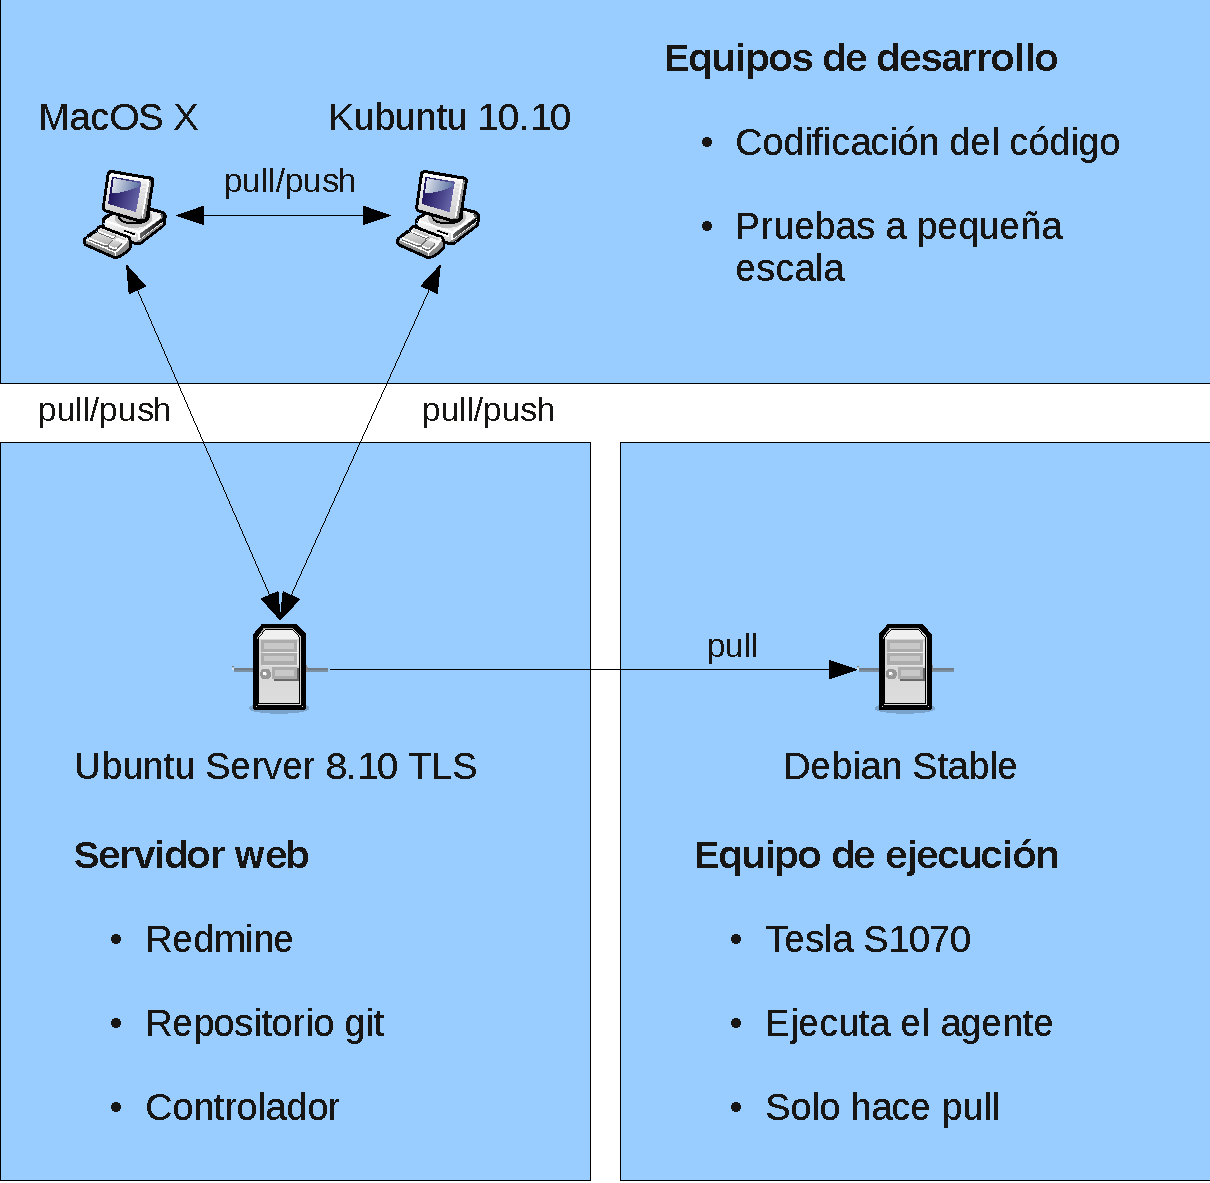
\includegraphics[width=0.7\textwidth]{images/entorno_trabajo.pdf}
	\caption{Diagrama del entorno de trabajo}\label{fig:entorno_trabajo}
\end{figure}
	\chapter{Manual de usuario} 

En el este capítulo se va a mostrar como instalar y usar DHC. Además se verán algunos detalles más avanzados de configuración para casos especiales.

\section{Instalación}

Antes de poder hacer uso de la aplicación es necesario instalarla. En las siguiente subsecciones se explicarán los pasos detallados para poner a punto el sistema.

\subsection{Instalación del agente}

El agente es uno de los elementos esenciales de DHC y el que entraña mayor dificultad de instalación. Por ese motivo hay que prestar especial detalle al procedimiento para identificar posibles fallos.

El proceso de instalacion consiste en la instalación del sistema operativo en la máquina, los controladores del mismo y las herramientas de compilación tal y como se ha descrito en el apéndice~\ref{chap:entorno}.

Una vez instalado todas las herramientas necesarias se procede a la compilación del agente. Para este propósito se deberán seguir los siguiente pasos:

\begin{enumerate}
	\item Se hace una copia del repositorio para trabajar con ella:
	
	\begin{verbatim}
	$ git clone $LOCATION dhc
	\end{verbatim}
	
	\$LOCATION hace referencia al lugar en el que se encuentre el repositorio y puede ser de la forma \emph{file://directorio} o \emph{usuario@ssh://direccion/ruta}. Una vez realizada esta copia dispondremos de una version local del respositorio sobre la que trabajar. Esta versión se habrá creado en el directorio en el que nos estuviéramos en el momento de realizar la llamada.
	
	\item Preparamos la compilación:
	
	\begin{verbatim}
	$ cd dhc/v3
	$ cmake .
	$ mkdir ptx
	\end{verbatim}
	
	\item Compilamos el código:
	
	\begin{verbatim}
	$ make
	\end{verbatim}
	
	\item Una vez compilado el código disponemos en el directorio del proyecto de una carpeta llamada \emph{bin} y otra \emph{ptx} que contienen los binarios del sistema operativo y de CUDA. Para terminar la instalación procederemos del siguiente modo:
	
	\begin{verbatim}
	$ sudo cp bin/agent /usr/bin
	$ sudo mkdir -p /usr/lib/cracker/ptx
	$ sudo cp bin/*.aplug.so /usr/lib/cracker/ptx
	$ sudo cp ptx/* /usr/lib/cracker/ptx
	\end{verbatim}
\end{enumerate}

En el cuadro~\ref{tab:mat_agente} podemos ver la lista de tareas a realizar. Este cuadro puede ser utilizado como \emph{checklist} de la instalación.

\begin{table}
	\centering
	
	\begin{tabular}{|c|p{5.6cm}|p{5.6cm}|}
	\hline
	Hecho & Descripción & Notas\\
	\hline
	& Instalar S.O. Linux en el ordenador & \\
	\hline
	& Instalar las herramientas de desarrollo de g++ y cmake & \\
	\hline
	& Comprobar e instalar, si es necesario, las cabeceras de Linux & \\
	\hline
	& Instalar controladores de NVIDIA con soporte de CUDA & \\
	\hline
	& Comprobar si se han creado los dispositivos de NVIDIA en /dev & \\
	\hline
	& Compilación del agente & \\
	\hline
	& Instalación de los binarios &\\
	\hline
	\end{tabular}
	
	\caption{Matriz de comprobación de la instalación del agente}\label{tab:mat_agente}
\end{table}

\subsection{Instalación de controlador}

El controlador es la parte encargada de la gestión del sistema. Es algo más sencilla de instalar que el agente al no requerir ninguna compilación, pero en cambio necesita que se modifiquen ciertos ficheros.

Para poder utilizar el controlador hace falta que el ordenador disponga del servidor web Apache y PHP. Además puede tener MySQL o se puede alojar la base de datos en otro ordenador. Con independencia de dónde se decida instalar MySQL se considerarán las siguiente variables que utilizaremos para identificar datos de configuración:

\begin{description}
	\item[PWEB] Ruta al punto en que se encontrará el controlador y que es un directorio accesible desde internet (normalmente es /var/www).

	\item[WEB\_HOST] Dirección del servidor web para la base de datos (si el servidor aloja ambos servicios se considerará que es localhost).

	\item[MYSQL\_HOST] Dirección IP de la máquina que aloja el servidor de base de datos (en caso de ser el mismo equipo que el servidor web se considerará que es localhost).

	\item[DB\_USER] Usuario que se configurará en MySQL para poder acceder a la base de datos del controlador.

	\item[DB\_PASS] Contraseña del usuario \$DB\_USER.

	\item[DB\_NAME] Nombre que tendrá la base de datos (por ejemplo, DHC).
\end{description}

Los pasos a seguir para la instalación son los siguientes:

\begin{enumerate}
	\item Instalar el sistema operativo en el servidor de Apache y de MySQL según lo mostrado en el apéndice~\ref{chap:entorno}.
	
	\item Creamos la base de datos en el servidor de MySQL:
	
	\begin{verbatim}
	$ mysql -h $MYSQL_HOST -u root -p
	mysql> create database $DB_NAME
	mysql> grant all privileges on $DB_NAME.* to `$DB_USER`@`$WEB_HOST` identified by '$DB_PASS'
	mysql> quit
	\end{verbatim}

	\item Se hace una copia del repositorio para trabajar con ella:
	
	\begin{verbatim}
	$ git clone $LOCATION dhc
	\end{verbatim}
	
	\$LOCATION hace referencia al lugar en el que se encuentre el repositorio y puede ser de la forma \emph{file://directorio} o \emph{usuario@ssh://direccion/ruta}. Una vez realizada esta copia dispondremos de una version local del respositorio sobre la que trabajar. Esta versión se habrá creado en el directorio en el que nos estuviéramos en el momento de realizar la llamada.

	\item Copiamos el controlador a su destino:
	
	\begin{verbatim}
	$ sudo cp -r dhc/v3/controller/* $PWEB
	\end{verbatim}
	
	\item Volcamos la base de datos inicial:
	
	\begin{verbatim}
	$ mysql -h $MYSQL_HOST -u $DB_USER \
	  -p $DB_PASS < $PWEB/app/config/database.sql
	\end{verbatim}
	
	\item Editamos el fichero de configuración de la base de datos (\$PWEB/app/config/database.php) para que quede como sigue:
	
	\begin{verbatim}
	class DATABASE_CONFIG {
	  var $default = array(
	    'driver' => 'mysql',
	    'persistent' => false,
	    'host' => '$MYSQL_HOST',
	    'login' => '$DB_USER',
	    'password' => '$DB_PASS',
	    'database' => '$DB_NAME',
	    'prefix' => '',
	  );

	  var $test = array(
	    'driver' => 'mysql',
	    'persistent' => false,
	    'host' => '$MYSQL_HOST',
	    'login' => '$DB_USER',
	    'password' => '$DB_PASS',
	    'database' => '$DB_NAME',
	    'prefix' => '',
	  );
	}
	\end{verbatim}
\end{enumerate}	

A partir de este momento el controlador ya se encuentra listo para ser utilizado. En el cuadro~\ref{tab:mat_controlador} podemos ver un resumen de los pasos a seguir.

\begin{table}
	\centering
	
	\begin{tabular}{|c|p{5.6cm}|p{5.6cm}|}
	\hline
	Hecho & Descripción & Notas\\
	\hline
	& Instalar S.O. Linux en el servidor web & \\
	\hline
	& Instalar S.O. Linux en el servidor de MySQL & \\
	\hline
	& Configurar MySQL & \\
	\hline
	& Copiamos e instalamos el controlador & \\
	\hline
	& Iniciamos la base de datos & \\
	\hline
	& Configuramos el acceso a la base de datos & \\
	\hline
	\end{tabular}
	
	\caption{Matriz de comprobación de la instalación del controlador}\label{tab:mat_controlador}
\end{table}

\section{Uso de DHC}

Para utilizar DHC se hace uso del controlador. Éste es la interfaz que permitirá utilizar todas las funcionalidades que nos ofrezcan los agentes. Pero antes de esto hay que iniciar los agentes.

La inicialización de un agente es tan sencilla como ejecutar el siguiente comando en el ordenador en que se encuentre:

\begin{verbatim}
$ agent $DIRECCION_CONTROLADOR
\end{verbatim}

Donde \$DIRECCION\_CONTROLADOR es la URL del controlador.

Una vez que se tiene a los agentes en funcionamiento se puede proceder a utilizar el controlador. Para este fin de hará uso de un navegador web\footnote{Actualmente existe una gran cantidad de navegadores web en el mercado. Se recomienda encarecidamente el uso de navegadores con soporte de HTML5 y CSS3 como pueden ser Google Chrome, Apple Safari o Mozilla Firefox.}

Nada más entrar en la aplicación podemos observar una pantalla como la mostrada en la figura~\ref{fig:DHC_principal}. En caso de que el sistema esté en funcionamiento podremos ver a qué velocidad está trabajando (en millones de hashes por segundo) o nada en otro caso.

\begin{figure}
	\centering
	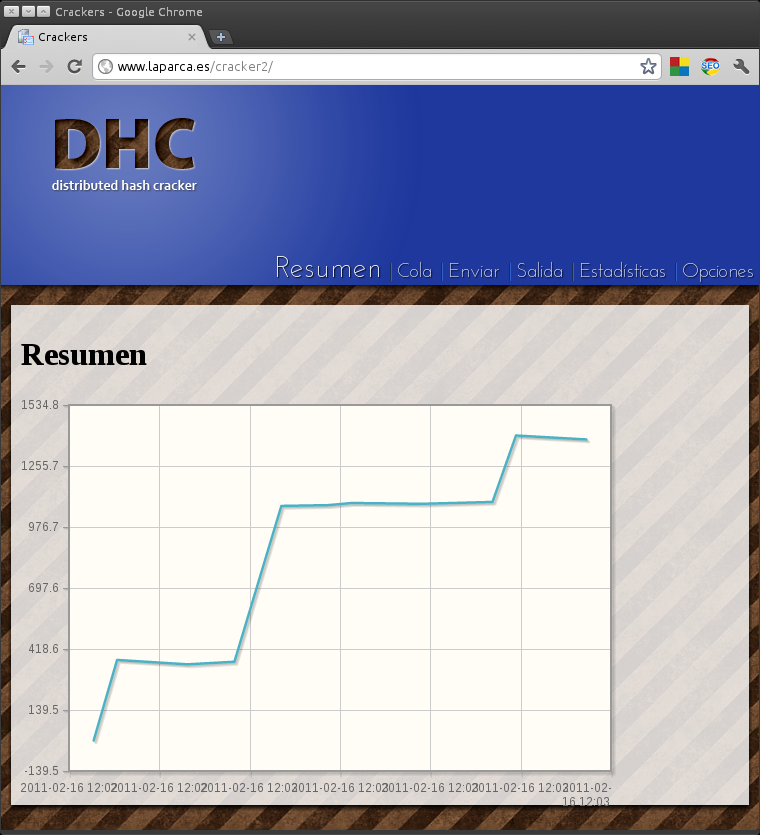
\includegraphics[width=0.7\textwidth]{images/resumen.png}
	\caption{Pantalla principal de DHC}\label{fig:DHC_principal}
\end{figure}

El primer paso es ir a enviar para solicitar la realialización de alguna tarea (ver figura~\ref{fig:DHC_enviar}). En este punto tendremos que seleccionar todas las opciones de configuración de la tarea.

\begin{figure}
	\centering
	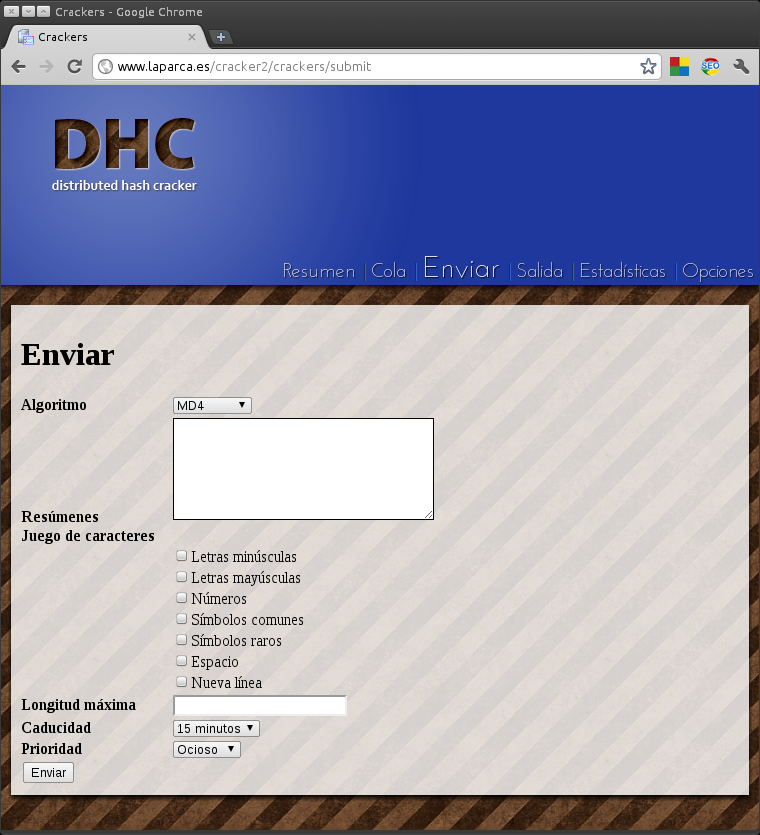
\includegraphics[width=0.7\textwidth]{images/dhc_enviar.png}
	\caption{Envío de una tarea}\label{fig:DHC_enviar}
\end{figure}

Tras el envío de la tarea el sistema nos dirá si ésta se ha almacenado correctamente o si a habido algún error.

En todo momento podemos comprobar qué tareas hay en funcionamiento desde la pantalla de cola (figura~\ref{fig:DHC_cola}).

\begin{figure}
	\centering
	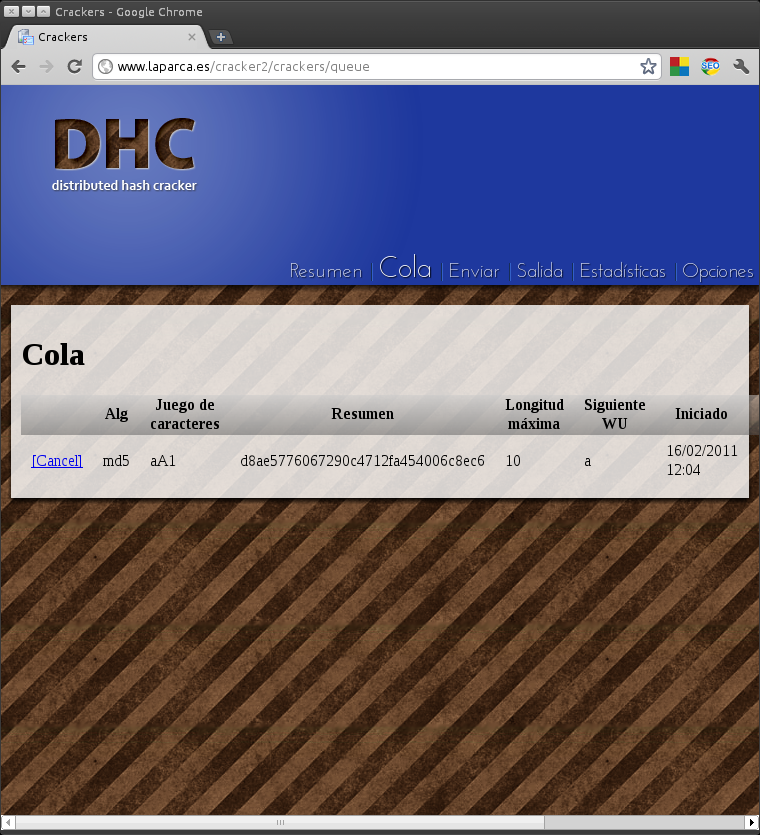
\includegraphics[width=0.7\textwidth]{images/cola.png}
	\caption{Cola de tareas}\label{fig:DHC_cola}
\end{figure}

Finalmente, podemos comprobar las tereas que se han terminado en la sección salida (ver figura~\reg{fig:DHC_salida}). Además, se puede comprobar la razón de la finalización de la tarea (resultado encontrado, no encontrado, etc.).

\begin{figure}
	\centering
	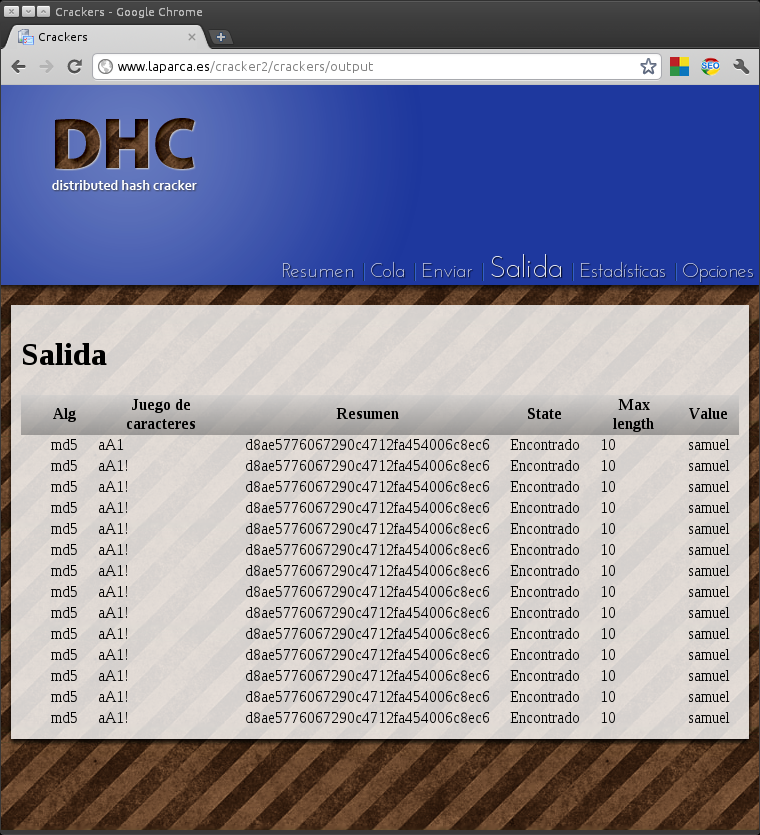
\includegraphics[width=0.7\textwidth]{images/salida.png}
	\caption{Salida de las tareas}\label{fig:DHC_saliad}
\end{figure}

Si en algún momento queremos conocer mejor la situación de los agentes, se puede comprobar en estadísticas (ver figura~\ref{fig:DHC_estadisticas}) el rendimiento de cada uno y el último momento en que se ha sabido de ellos.

\begin{figure}
	\centering
	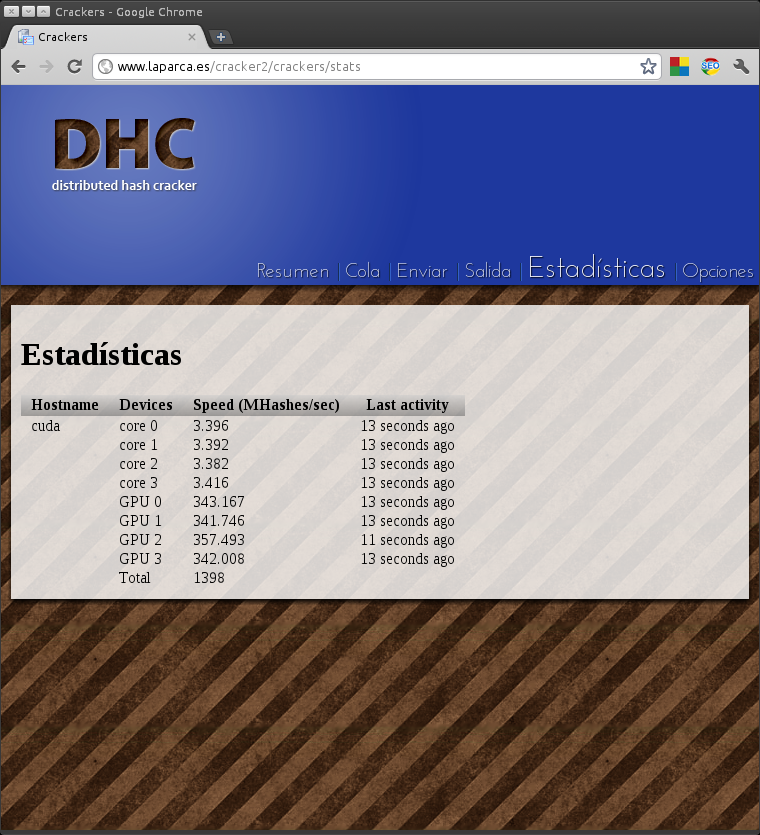
\includegraphics[width=0.7\textwidth]{images/estadisticas.png}
	\caption{Estadísticas de funcionamiento}\label{fig:DHC_estadisticas}
\end{figure}

\section{Administración de \emph{plugins}}

Durante el tiempo que esté en uso DHC pueden surgir ocasiones en las que se necesite instalar nuevos \emph{plugins} o eliminar los antiguos.  Para ello se seguirán los siguientes pasos en el agente sin olvidar que tras la modificación hay que reiniciar el agente.

\subsection{Instalación de nuevos plugins}

Para instalar nuevos plugins en el sistema solo hay que copiar estos al directorio /usr/lib/cracker/ptx. Los \emph{plugins} tienen todos la extensión .aplug.so.

\subsection{Eliminación plugins obsoletos o erróneos}

Para eliminar un \emph{plugin} con errores u obsoleto basta con borrar el fichero que lo contiene:

\begin{verbatim}
$ sudo rm /usr/local/cracker/ptr/nombre_plugin.aplug.so	
\end{verbatim}

\section{Configuraciones avanzadas}\label{sec:conf_avanzada}

En ciertas ocasiones puede hacer falta realizar instalaciones especiales de DHC. En esta sección se van a explicar dos opciones que hemos detectado.

\subsection{Varios controladores con un MySQL}
Puede darse el caso de que se necesite disponer de varios controladores de DHC pero que compartan una única base de datos. Esto puede resultar útil si la carga sobre un único controlador es muy elevada.

Para llevar a cabo este proceso se deben instalar dos o más controladores, solo con servidor web siguiendo los pasos descritos anteriormente, y a parte se configurará otro servidor con MySQL. Ambos controladores se configurarán para utilizar dicho servidor de MySQL.

Una vez que se inicien los agentes se irá pasando a cada uno la URL del controlador que deseemos o podemos configurar un balanceador de carga automático.


\subsection{Cambio de los tiempos de espera para evitar exceso de reciclado de WU}
En ciertas ocasiones, los agentes pueden tardar mucho en devolver el resultado de una WU por lo que se hace necesario modificar los tiempo de caducidad para evitar un exceso de reciclados que ralentizarían sobremedida el proceso de comprobación.

\subsection{Cambio de los directorios de búsqueda predeterminados}
Cuando un agente se inicia siempre comprueba la existencia de \emph{plugins} en unos directorios predefinidos. Además, también busca en estos mismos directorio los ficheros binarios de CUDA que le puedan ser solicitados por los algoritmos. Por defecto estos directorios son: el directorio desde el que se ejecuta el agente, el directorio \emph{ptx} desde el que se ejecuta el agente y el directorio \emph{/usr/lib/cracker/ptx}.

En caso de que se quisiese cambiar este comportamiento se puede editar el fichero config.cpp del agente para añadir o eliminar directorios de búsqueda.
	\chapter{Glosario}

\begin{description}
	\item[Algoritmo] Para el propósito de este proyecto un algoritmo es cualquier código destinado a poder ejecutarse en CPU o GPU con el fin de obtener una clave a partir de un conjunto de datos cifrados.
	
	\item[API] Aplication Programming Interface o interfaz de programación de aplicación. Es un conjunto de especificaciones destinadas a facilitar la realización de ciertas tareas.
	
	\item[Colision] Una colisión en el ámbito de las funciones resumen es cuando se dispone de dos mensajes diferentes que producen el mismo resumen.
	
	\item[Commit] Cada vez que se realizan modificaciones sobre fichero y se desea almacenar estas en el repositorio de versiones se realiza una operación de \emph{commit}.

	\item[CPU] \emph{Central Process Unit}. Es la unidad central de proceso y está encargada de ejecutar el código binario.
	
	\item[Distribución Linux] En el mundo del sistema operativo Linux se llama distribución a un paquete que contiene el núcleo Linux junto a un determinado conjunto de herramientas.
	
	\item[Fetch] Herramienta de git que permite consultar a un repositorio remoto por los cambios que han ocurrido. Estos cambios no se aplican localmente.
	
	\item[Framework] Conjunto de herramientas y especificaciones que permiten desarrollar aplicaciones de forma sencilla. La diferencia con el API es que esta última solo define bibliotecas para utilizar, mientras que el framework puede ir acompañado de herramientas.
	
	\item[GPU] \emph{Graphic Process Unit} o unidad de proceso gráfico es el procesador utilizado por una tarjeta gráfica para controlar las operaciones que se realizan sobre la misma. En la actualidad permiten la carga de programas de usuario especialmente diseñados.
	
	\item[HEAD] En git HEAD hace referencia a la última revisión que se encuentra en el repositorio.

	\item[Linux] Es un núcleo de sistema operativo que nació del núcleo Minix.
	
	\item[Makefile] Es un fichero que tiene las reglas a seguir para construir (compilar) un proyecto software.
	
	\item[MVC] Patrón arquitectónico Modelo-Vista-Controlador. Es una modo de organizar el código de tal forma que se diferencia claramente qué se encarga de la persistencia de datos (el modelo), qué se encarga del control de la lógica del programa (el controlador) y qué se encarga de presentar los datos al usuario (la vista).
	
	\item[Núcleo] En sistemas operativos el núcleo es un software que se encarga de facilitar los recursos del sistema a los programas.
	
	\item[Pull] En git se utiliza pull para aplicar a la rama actual de desarrollo que se encuentre activa los últimos cambios que se hayan hecho. Es recomendable hacer \emph{fetch} previamente.
	
	\item[Rack] Es un armario especial para poder poner equipos informáticos como ordenadores, switch, etc.
	
	\item[Rama de desarrollo] Es una líena de desarrollo de un proyecto en la que se hacen modificaciones. Las modificaciones realizadas en una rama no son vistas por el resto de ramas.
	
	\item[Push] Es el mandato que utiliza git para enviar todos los cambios locales a un repositorio remoto. Si no se indica ningún repositorio se utilizará el repositorio \emph{origin}.
	
%	\item[SLOC] \emph{Source Lines Of Code}. Son líneas de código fuente sin tener en cuenta los comentarios.
	
	\item[URL] Dirección de un elemento en internet. Suele estar definido por el tipo de protocolo, la dirección de la máquina y la ruta al elemento. Por ejemplo, http://www.google.com/reader. En este caso se accede a la máquina www.elpais.es utilizando el protocolo HTTP para solicitar /reader.
\end{description}

	\chapter{Códigos destacados} 

En este apéndice se van a presentarr los ficheros de código fuente que probablemente sean más interesantes en el proyecto. La mayoría representan únicamente aquellos ficheros que disponen de código importante sobre los cambios realizados.

Por otra parte se presenta también la organización de los ficheros para que en caso de acceder al código se sepa dónde se encuentra cada cosa.

\section{Organización del código}

El código fuente del proyecto se encuetra en la subcarpeta v3. En esta se puede encontrar la carpeta del agente, del controlador y la documentación:

\begin{enumerate}
	\item[v3/agent/] Código fuente del agente.

	\item[v3/controller/] Contiene el código fuente del controlador.
	
	\item[v3/controller/components/] Aquí se encuentran herramientas que son de utilidad para el desarrollo de la aplicación.

	\item[v3/controller/app/config/] Almacena la información de configuración de la base de datos y de algunas variables del controlador.

	\item[v3/controller/app/models] En esta carpeta se encuentra la definición del modelo de base de datos. Cada fichero representa una tabla.

	\item[v3/controller/app/views] La representación de los datos devueltos, tanto en la parte web como en los agente se lleva a cabo desde este punto.

	\item[v3/controller/app/controllers/] El control de las acciones se lleva a cabo en esta carpeta.

	\item[v3/doc] Código fuente de esta memoria.
\end{enumerate}

\section{Códigos importantes del agente}

\lstset{language=C++,tabsize=2,basicstyle=\tiny,numbers=left}

\putcode{agent/config.cpp}
\putcode{agent/Algorithm.h}
\putcode{agent/AlgorithmFactory.h}
\putcode{agent/AlgorithmFactory.cpp}
\putcode{agent/Executor.h}
\putcode{agent/ExecutorFactory.h}
\putcode{agent/ExecutorFactory.cpp}
\putcode{agent/Plugin.h}
\putcode{agent/PluginLoader.h}
\putcode{agent/PluginLoader.cpp}
\putcode{agent/debug.h}
\putcode{agent/DummyPlugin.h}
\putcode{agent/DummyPlugin.cpp}

\section{Códigos importantes del controlador}

\lstset{language=PHP}
\putcode{controller/app/controllers/crackers_controller.php}
\putcode{controller/app/controllers/agents_controller.php}
\putcode{controller/app/controllers/ajax_controller.php}
\putcode{controller/app/controllers/components/stats.php}
%\putcode{controller/app/controllers/components/base_n.php}
\subsection{v3/controller/app/controllers/components/base\_n.php}
\lstinputlisting{../../controller/app/controllers/components/base_n.php}}


	\chapter{Contenido del CD}

En el CD que se adjunta contiene los siguiente elementos:

\begin{description}
	\item[Document.pdf] Es la memoria del proyecto fin de carrera tal y como se encuentra impresa.
	
	\item[cracker/] Es una copia completa del respositorio de versiones. Contiene el código del agente, del controlador y la memoria además de todos los cambios que se han realizado desde el inicio del proyecto.
\end{description}
	\chapter{Aviso legal}

A pesar de no haberse utilizado las correspondientes marcas de copyright y marcas comerciales a lo largo de este texto, todos los nombre utilizados pertenecen a sus respectivos propietarios según la ley 17/2001, de 7 de diciembre, de Marcas.
	\chapter{Agradecimientos} 

La consecución de este proyecto no habría sido posible sin el apoyo y ayuda de mucha gente. Por este motivo desaría dedicar una agradecimiento a:

\begin{itemize}

	\item José María Sierra, porque sin su paciencia y dedicación al proyecto éste nunca habría podido ser posible.
	
	\item A mis amigos David, Victor y Paula, que aunque sé que no os he podido hacer mucho caso siempre estabais ahí cuando os necesitaba.
	
	\item A mis padres, por su apoyo a los largo de tantos años.
	
	\item A mi novia Sandra, que a pesar de saber que soy informático me quiere igual.
	
	\item A mis compañeros de física, por todas las risas que no echamos y por toda la ayuda que me han ofrecido.

\end{itemize}

Sé que me dejo a mucha gente en el tintero y espero que me lo podáis perdonar. Gracias a todos.

	\bibliographystyle{alpha}
	\bibliography{bibliografia}\addcontentsline{toc}{chapter}{Bibliografía}
\end{document}
